% \listoftodos
\chapter{Introduction}
In a forensic context, file recovery is a frequent task that can be motivated by several situations, like physical media malfunction, intentional attempt to hide data, and the need to access deleted or older versions of files. When the filesystem no longer provides the physical location of a file on the media, data carving is often the only procedure capable of retrieving its content.


    %\section{Motivation}
    Data carving is a forensic process that attempts to recover files without previous information of where the file starts or ends \cite{garfinkel_carving_2007}.
To accomplish this, a software has to analyze a source of raw data, searching for patterns indicating a known file type and making attempts to locate and reconstruct each of its constituent parts.
That process commonly disregards the filesystem \cite{veenman_statistical_2007}, being able to recover deleted files from unallocated areas, but faces the problem of fragmentation \cite{veenman_statistical_2007}  \cite{pal_evolution_2009}: in many cases, files are not written sequentially on disk and deleted files may have missing parts.

For example, while doing data carving on a hard drive, a software could sequentially read each drive sector, find a known header of a video file and save the following sectors until a footer is found or a size limit is reached. This is a common data carving approach, but one that fails to recover fragmented videos.

The patterns searched by data carving software are generally manually coded, taking advantage of fixed byte sequences found on headers and footers. But the amount of different file types combined with the slow process of manually coding each of those patterns makes the development of data carving software a tedious task \cite{mcdaniel_content_2003}.

The application of machine learning solutions to this manual task has the potential to make it easier and faster. The two tasks that could most likely benefit from the usage of machine learning techniques are file fragment classification and file reassembling. File fragment classification aims to identify the original type of file from which a given block of data was extracted. Reassembling is the attempt to reconstruct a file from pieces that may be out of order and mixed with pieces from other files.

Sequence labeling is a branch of machine learning that seeks to attribute labels to a sequence of instances related to each other.

This work describes the current state of art in data carving and in sequence labeling, exploring how neural networks can be applied in file fragment classification and reassembling.
    
    %\section{Document organization}
    
The remainder of this document is organized as follows.
    Chapter 2 analyses the current status of data carving tools and research. 
    Chapter 3 analyses the current status of sequence labeling research using neural networks.
    Chapter 4 analyses compares the accuracy of fourteen neural network models, mixing LSTM, fully-connected, and convolutional layers in the file fragment classification task.
    Chapter 5 presents the conclusion.


\chapter{Data carving}
\chapter{Data carving}
This chapter evaluates the data carving research field, with a focus on machine learning approaches. Section \ref{sec:data-carving-sms} describes a Systematic Mapping Study (SMS) focused on data carving, and Section \ref{sec:data-carving-taxonomies} lists some classifications schemes found in the literature.
% , Section \ref{sec:data-carving-existing-tools} discusses the technology gap between research and tools, and Section 
% \ref{sec:data-carving-challenges} consider some of the challenges of the data carving field.

A Systematic Mapping Study (SMS) is a secondary study performed to 
find and aggregate best available evidence on a specific topic \cite{petersen_systematic_2008}.

The employed background research methodology was inspired by PICO (Population, Intervention, Comparison, Outcome) criteria \cite{kitchenham_guidelines_2007}.

To assess the current research status on data carving machine learning technologies, the following research question was defined:

\begin{enumerate}[itemindent=\parindent,label=\textbf{RQ\arabic*.}]
    \item What machine learning algorithms have already been applied in the data carving field?
\end{enumerate}

To conduct the search, the following digital libraries were used: 
ACM (\url{https://dl.acm.org/}),
IEEE (\url{https://ieeexplore.ieee.org/}),
Scopus (\url{https://www.scopus.com/}),
and
Springer Link (\url{https://link.springer.com/}).

The terms chosen to address this question are shown in Table \ref{tab:dataterms}, resulting in the search strings presented in  Figure \ref{fig:datasearchstring}.

To choose those terms, generic expressions were used, to increase the number of results. But even using this strategy, the number of papers found was low. Comparison and Outcome terms were intentionally not used to avoid further reduction of results.

\begin{table*}[!ht]
    \centering
    \caption{Terms used}
    \label{tab:dataterms}
    \begin{tabular}{ l  l }
      Structure 	& Terms 		\\
      \hline\hline
      Population 	& data-carving \\   
                    & data carving \\
      \hline
      Intervention 	& machine learning \\
                    & neural networks \\
      \hline
    \end{tabular}
\end{table*}

\begin{figure}[!ht]
  \centering
  \fbox{\parbox{\textwidth}{\centering
    (``data carving'' AND ``machine learning'')\\
    (``data-carving'' AND ``machine learning'')\\
    (``data carving'' AND ``neural networks'')\\
    (``data-carving'' AND ``neural networks'')
  }}
  \caption{Search strings}
  \label{fig:datasearchstring}
\end{figure}


This initial approach brought few results, only four of which were considered relevant: \cite{alamri_taxonomy_2014}, 
\cite{ali_review_2018}, \cite{sportiello_context-based_2012}, and \cite{beebe_sceadan:_2013}. But using citations and references of these four works, the initial results were expanded and gave a more comprehensive view of current research on using machine learning techniques to perform data carving.

% In 2014, 
Alamri and Allen \cite{alamri_taxonomy_2014} created a taxonomy of file type identification techniques, grouped by the following broad categories: statistical learning, frequency distribution, statistical analysis, and detection of file fragments. The statistical learning category is subdivided in supervised and unsupervised leaning. The supervised learning techniques, which are the more relevant for this proposal, are Support Vector Machine (SVM), k-Nearest Neighbor (kNN), and Neural Network (NN). According to this taxonomy study, SVM is used in \cite{ahmed_fast_2011}, \cite{amirani_feature-based_2013}, \cite{beebe_sceadan:_2013}, \cite{fitzgerald_using_2012}, \cite{gopal_statistical_2011}, and \cite{sportiello_context-based_2012}, kNN is used in \cite{ahmed_fast_2011} and \cite{gopal_statistical_2011}, while neural networks are used in \cite{ahmed_fast_2011}, \cite{ahmed_content-based_2010}, \cite{amirani_new_2008}, \cite{amirani_feature-based_2013}, and \cite{penrose_approaches_2013}.

% In 2018, 
Ali et al. \cite{ali_review_2018} reviewed digital forensics methods for JPEG file carving. JPEG is mentioned in that paper as a common focus among data carving studies. Only some of the analyzed studies utilize some machine learning technique:
neural networks are used in \cite{xu_reassembling_2009} and \cite{amirani_feature-based_2013},
SVM is used in \cite{qiu_new_2014}, \cite{zhang_svm_2016}, and \cite{sportiello_file_2011},
kNN is used in \cite{axelsson_normalised_2010},
and Extreme Learning Machine (ELM) is used in \cite{zhang_svm_2016} and \cite{ali_classification_2018}.


Conti et al. \cite{conti_automated_2010} used kNN to classify low-level primitive types, like ASCII text, compressed data, bitmap, and encoded schemes.

According to Ali et al. \cite{ali_review_2018}, artificial intelligence techniques are found to be not fully utilized in this field. The relatively low research activity in the field could be an explanation for the research aspect of this observation.

% In 2005, 
Dunhan et al. \cite{dunham_classifying_2005} have successfully identified file type of encrypted files. First, they used a two-level neural network to identify files encrypted with the same key. Then, within each group of files, they used a three-level neural network to identify file types, using file deltas created with exclusive-or as input to the neural network. 

% In 2007, 
Harris \cite{harris_using_2007} described the attempt to use a neural network in data carving, but the neural networks tested were not considered better than the existing methods.

% In 2008, 
Amirami et al.  \cite{amirani_new_2008} used Principal Component Analysis (PCA) as input for a 5 layer feed-forward auto-associative unsupervised neural network to do feature extraction and a 3 layer Multi Layer Perceptron (MLP) to perform classification. They used a similar approach in 2013 \cite{amirani_feature-based_2013}. 
Among the studies found, this was the first to provide a viable alternative to classical data carving tools using a neural network approach. 
% 2013 work compared with svm

Other neural network works worth mentioning are:
% In 2009, 
Xu and Dong \cite{xu_reassembling_2009}, using a neural network as a cluster reassembling technique for JPEG image fragments;
% network structure not detailed
% In 2010, 
Ahmed et al. \cite{ahmed_content-based_2010}, using byte frequency as input to a neural network that performed file type classification and using a similar approach in their later work \cite{ahmed_fast_2011};
% In 2013, 
Penrose et al. \cite{penrose_approaches_2013}, using compression rate as the input to a neural network to distinguish between compressed and encrypted files;
% In 2014, 
Maslim et al. \cite{maslim_distributed_2014}, using Principal Component Analysis (PCA) of byte frequency distribution as input to a Gene Regulatory Engine (GRE) and a Distributed Adaptative Neural Network (DANN).
All these works applied some form of dimensionality reduction on the input data before performing classification.

% In 2018, 
Hiester \cite{hiester_file_2018} apparently was the first to utilize a LSTM network to perform file fragment classification. He compared results using three types of neural networks: feedforward, convolutional, and long short-term memory. The goal was to classify the data type of individual sectors (512 bytes), considering four file types: CSV, XML, JPG and GIF. For that, each bit was translated into two features, resulting in 8192 features per sector. First and last sectors of each file in the training set were discarded. In the experiments, the datasets were limited to one gigabyte to fit on memory.

Chen \textit{et al.} \cite{chen_file_2018}
used a Convolutional Neural Network (CNN) with 5 convolutional layers and 3 fully connected layers to classify fragments of 4096 bytes, converting each fragment into a 64x64 grayscale picture.

Wang \textit{et al.} \cite{wang_sparse_2018} 
used sparse dictionaries for n-grams to extract features of 512 bytes fragments, using this as input to an SVM classifier.
% They used 18 file types from the Govdocs1 dataset
% : csv, doc, docx, gif, gz, html, jpg, pdf, png, ppt, pptx, ps, rtf, swf, txt, xls, xlsx, and xml.

Wang \textit{et al.} \cite{wang_file_2018}  
compared CNN, SVM, kNN, and XGboost, with fragments of different sizes, converting each byte to a 256 length vector (one-hot encoding). The CNN combined 3 parallel convolutional layers of widths 4, 8, and 16.
They used 20 file types from the Govdocs1 dataset.
% : csv, doc, html, pdf, gif, jpg, dbase3, f, txt, swf, ps, java, log, xml, xls, ppt, gz, unk, rtf, and png.

Vulinović \textit{et al.} \cite{vulinovic_neural_2019}
compared a CNN with MLP, using 512 raw bytes as the CNN input, and byte histograms as input to the MLP.
% They used 18 file types from the Govdocs1 dataset
% : csv, doc, docx, gif, gz, html, jpg, pdf, png, ppt, pptx, ps, rtf, swf, txt, xls, xlsx, and xml.

Table \ref{tab:datacarvingstudies} summarizes the  machine learning techniques used in each data carving study.

\begin{table}[!ht]
\caption{Data carving studies using machine learning}
\label{tab:datacarvingstudies}
\begin{tabular}{l|c|c|c|c}

                                & \multicolumn{4}{c}{Technique} \\ \hline
Study                                     & SVM    & kNN    & NN   & ELM   \\ \hline
\hline
Dunham et al. \cite{dunham_classifying_2005} &        &        & x    &       \\ \hline
Harris \cite{harris_using_2007}              &        &        & x    &       \\ \hline
Amirani et al. \cite{amirani_new_2008}       &        &        & x    &       \\ \hline
Xu and Dong \cite{xu_reassembling_2009}      &        &        & x    &       \\ \hline
Ahmed et al. \cite{ahmed_content-based_2010} &        &        & x    &       \\ \hline
Axelsson \cite{axelsson_normalised_2010}     &        & x      &      &       \\ \hline
Conti et al. \cite{conti_automated_2010}     &        & x      &      &       \\ \hline
Ahmed et al. \cite{ahmed_fast_2011}          & x      & x      & x    &       \\ \hline
Gopal et al. \cite{gopal_statistical_2011}   & x      & x      &      &       \\ \hline
Sportiello and Zanero \cite{sportiello_file_2011} & x &        &      &       \\ \hline
Fitzgerald et al. \cite{fitzgerald_using_2012} & x    &        &      &       \\ \hline
Sportiello and Zanero \cite{sportiello_context-based_2012} & x  &  &  &       \\ \hline
Amirani et al. \cite{amirani_feature-based_2013} & x  &        & x    &       \\ \hline
Beebe et al. \cite{beebe_sceadan:_2013}      & x      &        &      &       \\ \hline
Penrose et al. \cite{penrose_approaches_2013} &       &        & x    &       \\ \hline
Qiu et al. \cite{qiu_new_2014}               & x      &        &      &       \\ \hline
Maslim et al. \cite{maslim_distributed_2014} &        &        & x    &       \\ \hline
Zhang et al. \cite{zhang_svm_2016}           & x      &        &      & x     \\ \hline
Ali et al. \cite{ali_classification_2018}    &        &        &      & x     \\ \hline
Hiester \cite{hiester_file_2018}             &        &        & x    &       \\ \hline
Chen et al. \cite{chen_file_2018}            &        &        & x    &       \\ \hline
Wang et al. \cite{wang_sparse_2018}          & x      &        &      &       \\ \hline
Wang et al. \cite{wang_file_2018}            & x      & x      & x    &       \\ \hline
Vulinović et al. \cite{vulinovic_neural_2019} &       &        & x    &       \\ \hline

\end{tabular}
\end{table}
\section{Data carving categories}
\label{sec:data-carving-taxonomies}

Ali et al. \cite{ali_review_2018} divide the data carving process in three steps:
    identification, which classifies the file type of individual chunks of data; 
    validation, which includes a list of requirements of a file that are needed for its recovery to be considered successful; and
    reassembling, which attempts to reconstruct the original file.

Some of the studies found deal only with the identification step, which has applications of its own, while others also include the challenge of achieving reassembling.

Nadeem \cite{nadeem_ashraf_forensic_2013} groups the carving techniques in three generations, each extending the previous one.
The first generation is a header-footer based carving. It uses file signatures like magic-bytes, headers, and footers to identify the beginning and end of a file.
The second generation is structure based carving, also called ``semantic carving'' or ``deep carving''. It reduces the number of false positives by using file structure knowledge to perform validation.
The third generation advances reassembling with methods to deal with fragmentation. It tries to infer relationships and order between chunks of data based on content and statistical analysis to reassemble the original file.

For file type detection, which could be mapped to the identification step in the  process steps of Ali et al. \cite{ali_review_2018}, Amirami et al. \cite{amirani_new_2008} cite three categories: extension-based identification, magic bytes-based identification, and content-based identification.
In extension-based identification, the content of the file is ignored and only its filename extension is used. Magic bytes-based identification uses signatures, generally a fixed string, usually at the beginning of a file. It is a common strategy that uses header/footer, but not all files adopt it. Content-based identification identifies the file using some statistical modeling of its content.

Beebe et al. \cite{beebe_sceadan:_2013} identify three content-based approaches to classify file and data types, also referring only to the identification step of the Ali et al. \cite{ali_review_2018} data carving process division: semantic parsing, nonsemantic parsing, and machine learning. Semantic parsing relies on the file structure to identify its type. Nonsemantic parsing searches for strings that are commonly found in specific files. Machine learning uses supervised and unsupervised algorithms, like Support Vector Machine (SVM), k-Nearest Neighbor (kNN), and Neural Networks (NN).

A summary of the categorization schemes is depicted on Table \ref{tab:categories}. As Nadeem \cite{nadeem_ashraf_forensic_2013} does not specifically mention machine learning, it is left out of generation classification.

\begin{table*}[!ht]
    \centering
    \caption{Data carving categories}
    \label{tab:categories}
    \begin{tabular}{ l | l | l | c }
      \multicolumn{3}{l|}{Steps}                                 & Generation\\
      \hline\hline
      Identification    & extension-based   &                   &   \\
                        \cline{2-3}
                        & magic bytes-based &                   & \multirow{-2}{*}{1\textsuperscript{st}}\\
                        \cline{2-4}
                        & content-based     & semantic          &   \\
                                            \cline{3-3}
                        &                   & non-semantic      & \multirow{-2}{*}{2\textsuperscript{nd}}\\
                                            \cline{3-4}
                        &                   & machine learning  &  --- \\
      \hline
      Validation        &                   &                   & 2\textsuperscript{nd} \\
      \hline
      Reassembling      &                   &                   & 3\textsuperscript{rd}\\
      \hline
    \end{tabular}
\end{table*}

% The available data carving tools generally do not take advantage of the latest techniques that research on the field offers, often still relying on header/footer identification and providing limited reassembling capabilities.

Some studies list available data carving tools
\cite{ali_review_2018}
\cite{qiu_new_2014}
\cite{nadeem_ashraf_forensic_2013}
\cite{roux_reconstructing_2008}, 
but the tool listing of Ali et al. \cite{ali_review_2018} is the most comprehensive. Among the listed tools, only Foremost \cite{kendall_foremost_2019}, Scalpel \cite{richard_iii_scalpel:_2005}, and PhotoRec \cite{grenier_photorec_2019} support a wide range of file formats. Photorec supports more than 300 file types. These three tools rely mainly on header/footer signature identification.

The amount of work required to support the vast amount of file types in existence is here chosen as a hypothesis for the reason for this discrepancy. Most of the attention paid to the results of data carving research is focused on increasing some statistical measurement of success, like accuracy. While these advances are undoubtedly important, they may not be the kind of research needed to transform these findings into practical tools. If this is the case, then the forensic community would benefit from researches that could make the task of supporting the carving of a new file type easier. Machine learning techniques have the potential to achieve that goal because it can replace the step of manually encoding a structure parser by automatically recognizing patterns in large amounts of data.

% \input{3.4-challenges.tex}




    \section{Systematic mapping study on data carving}
    \label{sec:data-carving-sms}
    A Systematic Mapping Study (SMS) is a secondary study performed to 
find and aggregate best available evidence on a specific topic \cite{petersen_systematic_2008}.

The employed background research methodology was inspired by PICO (Population, Intervention, Comparison, Outcome) criteria \cite{kitchenham_guidelines_2007}.

To assess the current research status on data carving machine learning technologies, the following research question was defined:

\begin{enumerate}[itemindent=\parindent,label=\textbf{RQ\arabic*.}]
    \item What machine learning algorithms have already been applied in the data carving field?
\end{enumerate}

To conduct the search, the following digital libraries were used: 
ACM (\url{https://dl.acm.org/}),
IEEE (\url{https://ieeexplore.ieee.org/}),
Scopus (\url{https://www.scopus.com/}),
and
Springer Link (\url{https://link.springer.com/}).

The terms chosen to address this question are shown in Table \ref{tab:dataterms}, resulting in the search strings presented in  Figure \ref{fig:datasearchstring}.

To choose those terms, generic expressions were used, to increase the number of results. But even using this strategy, the number of papers found was low. Comparison and Outcome terms were intentionally not used to avoid further reduction of results.

\begin{table*}[!ht]
    \centering
    \caption{Terms used}
    \label{tab:dataterms}
    \begin{tabular}{ l  l }
      Structure 	& Terms 		\\
      \hline\hline
      Population 	& data-carving \\   
                    & data carving \\
      \hline
      Intervention 	& machine learning \\
                    & neural networks \\
      \hline
    \end{tabular}
\end{table*}

\begin{figure}[!ht]
  \centering
  \fbox{\parbox{\textwidth}{\centering
    (``data carving'' AND ``machine learning'')\\
    (``data-carving'' AND ``machine learning'')\\
    (``data carving'' AND ``neural networks'')\\
    (``data-carving'' AND ``neural networks'')
  }}
  \caption{Search strings}
  \label{fig:datasearchstring}
\end{figure}


This initial approach brought few results, only four of which were considered relevant: \cite{alamri_taxonomy_2014}, 
\cite{ali_review_2018}, \cite{sportiello_context-based_2012}, and \cite{beebe_sceadan:_2013}. But using citations and references of these four works, the initial results were expanded and gave a more comprehensive view of current research on using machine learning techniques to perform data carving.

% In 2014, 
Alamri and Allen \cite{alamri_taxonomy_2014} created a taxonomy of file type identification techniques, grouped by the following broad categories: statistical learning, frequency distribution, statistical analysis, and detection of file fragments. The statistical learning category is subdivided in supervised and unsupervised leaning. The supervised learning techniques, which are the more relevant for this proposal, are Support Vector Machine (SVM), k-Nearest Neighbor (kNN), and Neural Network (NN). According to this taxonomy study, SVM is used in \cite{ahmed_fast_2011}, \cite{amirani_feature-based_2013}, \cite{beebe_sceadan:_2013}, \cite{fitzgerald_using_2012}, \cite{gopal_statistical_2011}, and \cite{sportiello_context-based_2012}, kNN is used in \cite{ahmed_fast_2011} and \cite{gopal_statistical_2011}, while neural networks are used in \cite{ahmed_fast_2011}, \cite{ahmed_content-based_2010}, \cite{amirani_new_2008}, \cite{amirani_feature-based_2013}, and \cite{penrose_approaches_2013}.

% In 2018, 
Ali et al. \cite{ali_review_2018} reviewed digital forensics methods for JPEG file carving. JPEG is mentioned in that paper as a common focus among data carving studies. Only some of the analyzed studies utilize some machine learning technique:
neural networks are used in \cite{xu_reassembling_2009} and \cite{amirani_feature-based_2013},
SVM is used in \cite{qiu_new_2014}, \cite{zhang_svm_2016}, and \cite{sportiello_file_2011},
kNN is used in \cite{axelsson_normalised_2010},
and Extreme Learning Machine (ELM) is used in \cite{zhang_svm_2016} and \cite{ali_classification_2018}.


Conti et al. \cite{conti_automated_2010} used kNN to classify low-level primitive types, like ASCII text, compressed data, bitmap, and encoded schemes.

According to Ali et al. \cite{ali_review_2018}, artificial intelligence techniques are found to be not fully utilized in this field. The relatively low research activity in the field could be an explanation for the research aspect of this observation.

% In 2005, 
Dunhan et al. \cite{dunham_classifying_2005} have successfully identified file type of encrypted files. First, they used a two-level neural network to identify files encrypted with the same key. Then, within each group of files, they used a three-level neural network to identify file types, using file deltas created with exclusive-or as input to the neural network. 

% In 2007, 
Harris \cite{harris_using_2007} described the attempt to use a neural network in data carving, but the neural networks tested were not considered better than the existing methods.

% In 2008, 
Amirami et al.  \cite{amirani_new_2008} used Principal Component Analysis (PCA) as input for a 5 layer feed-forward auto-associative unsupervised neural network to do feature extraction and a 3 layer Multi Layer Perceptron (MLP) to perform classification. They used a similar approach in 2013 \cite{amirani_feature-based_2013}. 
Among the studies found, this was the first to provide a viable alternative to classical data carving tools using a neural network approach. 
% 2013 work compared with svm

Other neural network works worth mentioning are:
% In 2009, 
Xu and Dong \cite{xu_reassembling_2009}, using a neural network as a cluster reassembling technique for JPEG image fragments;
% network structure not detailed
% In 2010, 
Ahmed et al. \cite{ahmed_content-based_2010}, using byte frequency as input to a neural network that performed file type classification and using a similar approach in their later work \cite{ahmed_fast_2011};
% In 2013, 
Penrose et al. \cite{penrose_approaches_2013}, using compression rate as the input to a neural network to distinguish between compressed and encrypted files;
% In 2014, 
Maslim et al. \cite{maslim_distributed_2014}, using Principal Component Analysis (PCA) of byte frequency distribution as input to a Gene Regulatory Engine (GRE) and a Distributed Adaptative Neural Network (DANN).
All these works applied some form of dimensionality reduction on the input data before performing classification.

% In 2018, 
Hiester \cite{hiester_file_2018} apparently was the first to utilize a LSTM network to perform file fragment classification. He compared results using three types of neural networks: feedforward, convolutional, and long short-term memory. The goal was to classify the data type of individual sectors (512 bytes), considering four file types: CSV, XML, JPG and GIF. For that, each bit was translated into two features, resulting in 8192 features per sector. First and last sectors of each file in the training set were discarded. In the experiments, the datasets were limited to one gigabyte to fit on memory.

Chen \textit{et al.} \cite{chen_file_2018}
used a Convolutional Neural Network (CNN) with 5 convolutional layers and 3 fully connected layers to classify fragments of 4096 bytes, converting each fragment into a 64x64 grayscale picture.

Wang \textit{et al.} \cite{wang_sparse_2018} 
used sparse dictionaries for n-grams to extract features of 512 bytes fragments, using this as input to an SVM classifier.
% They used 18 file types from the Govdocs1 dataset
% : csv, doc, docx, gif, gz, html, jpg, pdf, png, ppt, pptx, ps, rtf, swf, txt, xls, xlsx, and xml.

Wang \textit{et al.} \cite{wang_file_2018}  
compared CNN, SVM, kNN, and XGboost, with fragments of different sizes, converting each byte to a 256 length vector (one-hot encoding). The CNN combined 3 parallel convolutional layers of widths 4, 8, and 16.
They used 20 file types from the Govdocs1 dataset.
% : csv, doc, html, pdf, gif, jpg, dbase3, f, txt, swf, ps, java, log, xml, xls, ppt, gz, unk, rtf, and png.

Vulinović \textit{et al.} \cite{vulinovic_neural_2019}
compared a CNN with MLP, using 512 raw bytes as the CNN input, and byte histograms as input to the MLP.
% They used 18 file types from the Govdocs1 dataset
% : csv, doc, docx, gif, gz, html, jpg, pdf, png, ppt, pptx, ps, rtf, swf, txt, xls, xlsx, and xml.

Table \ref{tab:datacarvingstudies} summarizes the  machine learning techniques used in each data carving study.

\begin{table}[!ht]
\caption{Data carving studies using machine learning}
\label{tab:datacarvingstudies}
\begin{tabular}{l|c|c|c|c}

                                & \multicolumn{4}{c}{Technique} \\ \hline
Study                                     & SVM    & kNN    & NN   & ELM   \\ \hline
\hline
Dunham et al. \cite{dunham_classifying_2005} &        &        & x    &       \\ \hline
Harris \cite{harris_using_2007}              &        &        & x    &       \\ \hline
Amirani et al. \cite{amirani_new_2008}       &        &        & x    &       \\ \hline
Xu and Dong \cite{xu_reassembling_2009}      &        &        & x    &       \\ \hline
Ahmed et al. \cite{ahmed_content-based_2010} &        &        & x    &       \\ \hline
Axelsson \cite{axelsson_normalised_2010}     &        & x      &      &       \\ \hline
Conti et al. \cite{conti_automated_2010}     &        & x      &      &       \\ \hline
Ahmed et al. \cite{ahmed_fast_2011}          & x      & x      & x    &       \\ \hline
Gopal et al. \cite{gopal_statistical_2011}   & x      & x      &      &       \\ \hline
Sportiello and Zanero \cite{sportiello_file_2011} & x &        &      &       \\ \hline
Fitzgerald et al. \cite{fitzgerald_using_2012} & x    &        &      &       \\ \hline
Sportiello and Zanero \cite{sportiello_context-based_2012} & x  &  &  &       \\ \hline
Amirani et al. \cite{amirani_feature-based_2013} & x  &        & x    &       \\ \hline
Beebe et al. \cite{beebe_sceadan:_2013}      & x      &        &      &       \\ \hline
Penrose et al. \cite{penrose_approaches_2013} &       &        & x    &       \\ \hline
Qiu et al. \cite{qiu_new_2014}               & x      &        &      &       \\ \hline
Maslim et al. \cite{maslim_distributed_2014} &        &        & x    &       \\ \hline
Zhang et al. \cite{zhang_svm_2016}           & x      &        &      & x     \\ \hline
Ali et al. \cite{ali_classification_2018}    &        &        &      & x     \\ \hline
Hiester \cite{hiester_file_2018}             &        &        & x    &       \\ \hline
Chen et al. \cite{chen_file_2018}            &        &        & x    &       \\ \hline
Wang et al. \cite{wang_sparse_2018}          & x      &        &      &       \\ \hline
Wang et al. \cite{wang_file_2018}            & x      & x      & x    &       \\ \hline
Vulinović et al. \cite{vulinovic_neural_2019} &       &        & x    &       \\ \hline

\end{tabular}
\end{table}
    
    \section{Data carving categories}
    \label{sec:data-carving-taxonomies}
    \section{Data carving categories}
\label{sec:data-carving-taxonomies}

Ali et al. \cite{ali_review_2018} divide the data carving process in three steps:
    identification, which classifies the file type of individual chunks of data; 
    validation, which includes a list of requirements of a file that are needed for its recovery to be considered successful; and
    reassembling, which attempts to reconstruct the original file.

Some of the studies found deal only with the identification step, which has applications of its own, while others also include the challenge of achieving reassembling.

Nadeem \cite{nadeem_ashraf_forensic_2013} groups the carving techniques in three generations, each extending the previous one.
The first generation is a header-footer based carving. It uses file signatures like magic-bytes, headers, and footers to identify the beginning and end of a file.
The second generation is structure based carving, also called ``semantic carving'' or ``deep carving''. It reduces the number of false positives by using file structure knowledge to perform validation.
The third generation advances reassembling with methods to deal with fragmentation. It tries to infer relationships and order between chunks of data based on content and statistical analysis to reassemble the original file.

For file type detection, which could be mapped to the identification step in the  process steps of Ali et al. \cite{ali_review_2018}, Amirami et al. \cite{amirani_new_2008} cite three categories: extension-based identification, magic bytes-based identification, and content-based identification.
In extension-based identification, the content of the file is ignored and only its filename extension is used. Magic bytes-based identification uses signatures, generally a fixed string, usually at the beginning of a file. It is a common strategy that uses header/footer, but not all files adopt it. Content-based identification identifies the file using some statistical modeling of its content.

Beebe et al. \cite{beebe_sceadan:_2013} identify three content-based approaches to classify file and data types, also referring only to the identification step of the Ali et al. \cite{ali_review_2018} data carving process division: semantic parsing, nonsemantic parsing, and machine learning. Semantic parsing relies on the file structure to identify its type. Nonsemantic parsing searches for strings that are commonly found in specific files. Machine learning uses supervised and unsupervised algorithms, like Support Vector Machine (SVM), k-Nearest Neighbor (kNN), and Neural Networks (NN).

A summary of the categorization schemes is depicted on Table \ref{tab:categories}. As Nadeem \cite{nadeem_ashraf_forensic_2013} does not specifically mention machine learning, it is left out of generation classification.

\begin{table*}[!ht]
    \centering
    \caption{Data carving categories}
    \label{tab:categories}
    \begin{tabular}{ l | l | l | c }
      \multicolumn{3}{l|}{Steps}                                 & Generation\\
      \hline\hline
      Identification    & extension-based   &                   &   \\
                        \cline{2-3}
                        & magic bytes-based &                   & \multirow{-2}{*}{1\textsuperscript{st}}\\
                        \cline{2-4}
                        & content-based     & semantic          &   \\
                                            \cline{3-3}
                        &                   & non-semantic      & \multirow{-2}{*}{2\textsuperscript{nd}}\\
                                            \cline{3-4}
                        &                   & machine learning  &  --- \\
      \hline
      Validation        &                   &                   & 2\textsuperscript{nd} \\
      \hline
      Reassembling      &                   &                   & 3\textsuperscript{rd}\\
      \hline
    \end{tabular}
\end{table*}

    
    % \section{Existing tools}
    \label{sec:data-carving-existing-tools}
    The available data carving tools generally do not take advantage of the latest techniques that research on the field offers, often still relying on header/footer identification and providing limited reassembling capabilities.

Some studies list available data carving tools
\cite{ali_review_2018}
\cite{qiu_new_2014}
\cite{nadeem_ashraf_forensic_2013}
\cite{roux_reconstructing_2008}, 
but the tool listing of Ali et al. \cite{ali_review_2018} is the most comprehensive. Among the listed tools, only Foremost \cite{kendall_foremost_2019}, Scalpel \cite{richard_iii_scalpel:_2005}, and PhotoRec \cite{grenier_photorec_2019} support a wide range of file formats. Photorec supports more than 300 file types. These three tools rely mainly on header/footer signature identification.

The amount of work required to support the vast amount of file types in existence is here chosen as a hypothesis for the reason for this discrepancy. Most of the attention paid to the results of data carving research is focused on increasing some statistical measurement of success, like accuracy. While these advances are undoubtedly important, they may not be the kind of research needed to transform these findings into practical tools. If this is the case, then the forensic community would benefit from researches that could make the task of supporting the carving of a new file type easier. Machine learning techniques have the potential to achieve that goal because it can replace the step of manually encoding a structure parser by automatically recognizing patterns in large amounts of data.

    

\chapter{Machine learning applied to data carving}
\chapter{Machine learning applied to data carving}

% \section{Machine learning overview}
% tipos de aprendizado
%  supervisionado
%   aplicacao a data carving
%    reconhecimento de arquivos
%    reconhecimento de setores avulsos
%    reconhecimento de estruturas 
%  nao supervisionado
%   agrupamento de setores
%   desfragmentação?
%  semi-supervisionado?
%  reinforcement?
%   talvez não aplicavel; descricao assistida de estruturas?

% tipos de funcao de erro
%  probabilidade
%   generative learning
%  classes
%   discriminative learning

The data carving field, despite being actively studied, does not have the number of research papers that other fields have. This implies that improvements in current data carving techniques are likely to use knowledge transferred from other areas. While in a machine learning search the excess of relevant papers becomes a problem, an equivalent data carving search may face a scarcity of relevant papers.

But, in order to find a field of study that describes the data carving problem in a more generic manner, the correct terminology must be used. Essentially, data carving could be described as a  ``pattern recognition'' problem, but this term is almost as broad as ``machine learning'', as some of the unsuccessful first search attempts showed. Using ``automatic pattern recognition'' was a slight improvement, but still not precise enough.

The interpretation of the inner structure of a file is usually done by parsers, which use a representation of that structure to extract or transform the file's content. But bibliography on parsers generally refers to language parsers, dealing with questions not entirely applicable to data carving, which is why the searches using the term ``parser'' were also unsuccessful.

% \todo[inline]{book?}
Although it is not good practice to use Wikipedia as a source of scientific research, it is arguably an acceptable starting point to gather terms referring to broad fields of study. With that reasoning, a Wikipedia search was conducted to find a better term to the problem. Several pages related to machine learning were read, in an empirical search for links that could lead to a potential better term. The most useful result was found at \url{https://en.wikipedia.org/wiki/Pattern\_recognition} \cite{wikipedia_pattern_2018}, giving the following glossary of pattern recognition algorithms:
    % classification algorithms,
    % clustering algorithms,
    % ensemble learning algorithms,
    % general algorithms for predicting arbitrarily-structured
    % sets of labels,
    % multilinear subspace learning algorithms,
    % real-valued sequence labeling algorithms,
    % regression algorithms, and
    % sequence labeling algorithms.
% \begin{itemize}
    classification algorithms,
    which are supervised algorithms predicting categorical labels, clustering algorithms,
    which are unsupervised algorithms predicting categorical labels,
    ensemble learning algorithms,
    which are supervised meta-algorithms for combining multiple learning algorithms together,
    multilinear subspace learning algorithms,
    that predict labels of multidimensional data using tensor representations,
    real-valued sequence labeling algorithms,
    that predict sequences of real-valued labels,
    regression algorithms, 
    that predict real-valued labels,
    and sequence labeling algorithms, 
    that predict sequences of categorical labels.
% \end{itemize}

% \todo[inline]{review this}
It is important to notice that different classes of algorithms would be suitable for different learning objectives.
A clustering algorithm could be used to group fragments of data with unknown structure.
A classification algorithm could be used to attribute labels to each disk sector, which is related to the identification step of data carving. 
Sequence labeling was the algorithm class selected to be further studied, as it considers relations between labels on a sequence, which is often the case when classifying consecutive sectors of a disk. This could lead to better classification and to reassembling of fragmented data.

Sequence labeling deals with the task of attributing categorical labels to a group of instances where, unlike happens with other classification problems, those instance labels are not independent.
One example of such task is known as Part Of Speech (POS) tagging, where the goal is, given a word in a sentence, classify it, for example as a noun or a verb.
The classification of each word is not independent of its surroundings since it provides context from which the meaning of the word may be inferred.

Another example of a sequence labeling task is found in speech recognition.
The sound of a spoken sentence is split into parts and each part receives a label corresponding to a phoneme. But those labels are not independent since some combinations of phonemes are meaningful while others are not. Thus, taking this context into account increases the accuracy of the results.

From those classes of pattern recognition approaches mentioned above, both classification algorithms and sequence labeling algorithms are good choices.
The difference is that the plain classification method should be easier to implement, while the sequence labeling method is expected to predict the labels better.

Another reason to choose sequence labeling over plain classification is to study if it is possible to extract structure insights from the models, leading to developments in information extraction.

In this section we describe the SMS used to find relevant work on sequence labeling (see section 2.1).

To search relevant studies about sequence labeling that could be applied in the data carving field, the following research questions were defined:

\begin{enumerate}[itemindent=\parindent,label=\textbf{RQ\arabic*.}]
\item   What are the sequence labeling algorithms used to treat unstructured data?
\item   In which application areas are they used?
\item   How do these algorithms compare to each other?
\item   Which of them could produce better results in data carving?
\end{enumerate}

To conduct the search, the following digital libraries were used: ACM (\url{https://dl.acm.org/}), 
IEEE (\url{https://ieeexplore.ieee.org/}),
Scopus (\url{https://www.scopus.com/}),
and
Springer Link (\url{https://link.springer.com/}).

The terms chosen to address those questions are shown in Table \ref{tab:terms}, grouped by research structure using the boolean operation “OR”, then globally combined using the boolean operation “AND”, resulting in the search string presented in  Figure \ref{fig:searchstring}.

To choose these terms, the abbreviations of some common techniques applied in sequence labeling were used, assuming it would be unlikely that a new technique would not mention one of these. 


\begin{table*}[!ht]
    \centering
    \caption{Terms used}
    \label{tab:terms}
    \begin{tabular}{ l  l  }
      Structure 	& Terms 		 \\
      \hline\hline
      Population 	& unstructured data \\   
                    & sequential data \\
      \hline
      Intervention 	& CNN (Convolutional Neural Networks)\\
                    & RNN (Recurrent Neural Networks)\\
                    & HMM (Hidden Markov Models)\\
                    & CRF (Conditional Random Fields)\\
                    & MEMM (Maximum-entropy Markov Models)\\
                    & DTW (Dynamic Time Warping)\\
      \hline
      Outcome 		& sequence labeling \\
      \hline
    \end{tabular}
\end{table*}

\begin{figure}[!ht]
  \centering
  \fbox{\parbox{\textwidth}{
    ("unstructured data"
    OR "sequential data"
    ) AND (
    "CNN"
    OR "RNN"
    OR "HMM"
    OR "CRF"
    OR "MEMM"
    OR "DTW"
    ) AND (
    "sequence labeling"
    )
  }}
  \caption{Search string}
  \label{fig:searchstring}
\end{figure}
	
The submission of the search string to the four mentioned databases returned 197 papers.
Results with unavailable content were ignored.
With the exclusion of 6 duplicated studies, title and abstract of 191 of them were read, resulting in 68 accepted papers in the intermediary selection, which required enough detail to implement the solution, some form of technique improvement, and the possibility of application on the data carving field.
Next, 47 of the papers were excluded after quality assessment, focused on eliminating redundant studies, resulting in 21 selected studies.

Table 
\ref{tab:results}
shows the total remaining studies from each database.


\begin{table}[!ht]
    \centering
    \caption{Search engines and selected studies at each phase.}
    \label{tab:results}
    \begin{tabular}{l r r r r}
    \hline
    Database &        Retrieved & 
                                Not duplic. & 
                                         Interm. Selection & 
                                               Final Selection\\
    \hline
    ACM	DL			& 40 &      40 &     12  & 5 \\
    IEEE Explore	& 72 &      72 &     24  & 7 \\
    Scopus			& 37 &      31 &     22  & 6 \\
    Springer Link	& 48 &      48 &     10  & 3 \\
    \hline
    Total           & 197 &    191 &     68  & 21 \\
    \hline
    
    \end{tabular}
\end{table}

The conclusions drawn from those studies are presented next, answering the formulated questions:

\newpage
\begin{enumerate}[listparindent=\parindent,itemindent=\parindent,label=\textbf{RQ\arabic*.}]
\item   \textbf{What are the sequence labeling algorithms used to treat unstructured data?}

Two groups of algorithms were identified as the most cited in sequence labeling: Conditional Random Fields (CRF) and Long Short-Term Memory (LSTM). 
Other algorithms found were Hidden Markov Models (HMM), to which CRF is related, some neural networks variants, from which LSTM is a subgroup, and Bidirectional Long Short-Term Memory (BLSTM), which is a variant of LSTM. 
Some algorithms are variations of others and some are hybrids, such as the combination of CRF and neural networks, and some were used only as baselines.

From the selected studies,
3 of them offer a broad overview of sequence labeling or machine learning: Graves \cite{graves_supervised_2012}, Deng and Li \cite{deng_machine_2013}, and Schmidhuber \cite{schmidhuber_deep_2015}.
    Graves \cite{graves_supervised_2012} provides an excellent overview of sequence labeling.
    Deng and Li \cite{deng_machine_2013} offer an overview of machine learning in general, which can be used to situate sequence labeling among other problems and to compare different techniques that have different goals and assumptions. 
    Schmidhuber \cite{schmidhuber_deep_2015} gives a detailed historical overview of machine learning.

The only selected study that don't apply CRF or neural networks was Daf{\'e} et al. \cite{dafe_learning_2015}, describing the approximately-contiguous sequential classifier (AC-SC) and pattern silhouettes, comparing it to HMM and other algorithms.

    
Conditional Random Fields (CRF) without neural networks are discussed in 
6 selected studies:
    % Cuong et al. \cite{Cuong:2014:CRF:2627435.2638567},
    % Chatzis and Demiris \cite{Chatzis20131523},
    % Wang and Zhang \cite{6213103}, Song et al. \cite{6247918},
    % Papadopoulos and Tzanetakis \cite{7579173},
    % and
    % Jeong and Lee \cite{4599397}.
    Cuong et al. \cite{cuong_conditional_2014} discuss high-order dependencies in CRF;
    Chatzis and Demiris \cite{chatzis_infinite-order_2013} discuss infinite order CRF;
    Wang and Zhang \cite{wang_ica_2013} describe Hidden Conditional Random Fields (HCRF);
    Song et al. \cite{song_multi-view_2012} describe Multi-View Latent Variable Discriminative Conditional Random Fields (MV-LDCRF);
    Papadopoulos and Tzanetakis \cite{papadopoulos_models_2017} compare HMM and CRF;
    Jeong and Lee \cite{jeong_triangular-chain_2008} explain triangular-chain CRF.

Neural Networks were used in 
11 of the selected studies.
From these, 
only 
4 do not use Long Short-Term Memory (LSTM): 
    Irsoy and Cardie \cite{irsoy_opinion_2014} compare CRF to Recurrent Neural Networks (RNN);
    Zhang et al. \cite{zhang_nonrecurrent_2017} describe compact Feedforward Sequential Memory Network (cFSMN);
    Zhao et al. \cite{zhao_recurrent_2017} describe Recurrent Convolutional Neural Network (RCNN) and compare it with LSTM;
    Cui et al. \cite{cui_continuous_2016} describe the Hierarchical Temporal Memory (HTM) sequence memory model, a neural network model that can do continuous online learning, and compares it with LSTM and other techniques.

The remaining 
7 studies use LSTM, where 
    Nguyen et al. \cite{nguyen_recurrent_2018} compare CRF to some combined models of CRF and BLSTM;
    Xie et al. \cite{xie_fully_2016} describe Fully Convolutional Recurrent Network (FCRN) combining a convolutional network with a multi-layer BLSTM;
    Fang et al. \cite{fang_deepasl:_2017} describe Hierarchical Bidirectional Deep Recurrent Neural Network (HB-RNN), which uses a tree of BLSTM networks;
    Veli\v{c}kovi\'{c} et al. \cite{velickovic_cross-modal_2018} describe Cross-modal LSTM (X-LSTM), which is a network of LSTMs;
    Tjandra et al. \cite{tjandra_gated_2016} combine LSTM with Gated Recurrent Unit (GRU) using tensor products;
    Liu et al. \cite{liu_global_2017} propose the Global Context Aware Attention LSTM (GCA-LSTM), that adds a global context memory block to LSTM;
    Feng et al. \cite{feng_attention_2018} add context attention layers to a hierarchical LSTM to produce a Context Attention LSTM (CA-LSTM).

\item   \textbf{In which application areas they are used?}

 The following are
 frequently seen areas 
 in which sequence label was applied 
 on the selected studies:
    Part Of Speech (POS) tagging, which
    associates part of speech labels to words in a sentence
    \cite{chatzis_infinite-order_2013}
    \cite{tjandra_gated_2016};
    speech recognition, which
    converts spoken words into text
    \cite{zhang_nonrecurrent_2017} \cite{zhao_recurrent_2017}
    \cite{graves_supervised_2012} 
    \cite{deng_machine_2013};
    handwriting recognition, which
    digitally transcribes a handwritten text
    \cite{cuong_conditional_2014}
    \cite{chatzis_infinite-order_2013}
    \cite{xie_fully_2016};
    protein sequence analysis, which
    compares regions of DNA or RNA with known protein sequences
    \cite{dafe_learning_2015};
    action recognition, which
    gives labels to predefined sequences of human motion, commonly translating body postures and hand shapes to commands or words
    \cite{song_multi-view_2012}
    % \item video segmentation
    \cite{chatzis_infinite-order_2013}
    % \item video event classification
    \cite{wang_ica_2013}
    % \item Gesture recognition:
    \cite{liu_global_2017}
    % \item sign language
    \cite{fang_deepasl:_2017};
    information extraction, which
    retrieves structured information from unstructured data, often text 
    % \item bibliography extraction
    \cite{cuong_conditional_2014}
    % \item opinion mining
    \cite{irsoy_opinion_2014}
    % \item legal texts
    \cite{nguyen_recurrent_2018}
    % sentiment classification
    \cite{feng_attention_2018}
    \cite{dafe_learning_2015}.

\item   \textbf{How do these algorithms compare to each other?}

% \begin{itemize}
    % \item HMM and CRF: 
    
    As explained by Papadopoulos and Tzanetakis \cite{papadopoulos_models_2017}, HMM and CRF are both cases of Markov Networks, but they differ in some aspects.
    % \begin{itemize}
        % \item 
        HMM represents $p(y,x)$ while CRF represents $p(y|x)$ (where $x$ is an observation and $y$ the label), which is why HMM is considered a generative model and CRF a discriminative one.
        Graves \cite{graves_supervised_2012} clarifies that $p(x)$, which can be obtained by $p(x) = \sum_{y} p(x,y)$, can be used to generate artificial data, hence the name.
        % \item 
        HMM assumes strong independence between observation variables while CRF relaxes that assumption.
        % \item 
        CRF generally gives better results than HMM in many real-world problems where the dependence between observation variables is common, like natural language processing, music audio signal processing, speech recognition, and bioinformatics.
        
    % \end{itemize}
    
    % \item High-order CRF:
    
    As Cuong et al. \cite{cuong_conditional_2014} detail, the common linear-chain CRF considers dependencies between at most two adjacent labels, because its computational cost is exponential in respect to the number of considered neighbors.
    
    Cuong et al. \cite{cuong_conditional_2014} approach to build high-order dependency relies on label sparsity, which happens when a sequence of repeated labels is a common occurrence.
    
    To achieve higher order dependency, Chatzis and Demiris \cite{chatzis_infinite-order_2013} combine CRF with a sequence memoizer, which is a non-Markovian model since it can consider all previous sequence values.
    
    % Wang and Zhang \cite{6213103} describes Hidden Conditional Random Fields (HCRF), 
    % Song et al. \cite{6247918} describes Multi-View Latent variable Discriminative Conditional Random Fields (MV-LDCRF),
    % Jeong and Lee \cite{4599397} explain triangular-chain CRF.
    
    
    % \item CRF and neural networks:
    
    Two studies compared CRF with some form of neural network, both giving an edge to neural networks over CRF.
    Irsoy and Cardie \cite{irsoy_opinion_2014} compared CRF and RNN, obtaining better F1-scores with RNN.
    Nguyen et al. \cite{nguyen_recurrent_2018} compared CRF to some combined models of CRF and BLSTM, obtaining better F1-scores with the BLSTM-CRF models.
    
    % \item Recurrent neural networks (RNN) and LSTM:
    
    As Graves \cite{graves_supervised_2012} explains, is very difficult for a standard RNN to retain information for longs periods of time because, with time, new data from the input layer tends to prevail over signals from the hidden layer, while LSTM has special `memory cells', which can retain information as long as necessary.
    
    Graves \cite{graves_supervised_2012} compared BLSTM, Bidirectional Recurrent Neural Network (BRNN) and Multilayer Perceptron (MLP). Compared with the other two, BLSTM produced better results in fewer epochs.
    
    Zhang et al. \cite{zhang_nonrecurrent_2017} 
    propose a nonrecurrent neural network model with a memory block and obtain better results in less time compared to BLSTM.

    Zhao et al. \cite{zhao_recurrent_2017} 
    report that RNNs are hard to train because they cannot take full advantage of GPUs, while Convolutional Neural Networks (CNN) do not improve speech recognition results compared to other techniques.
    Comparing the proposed model RCNN with LSTM, RCNN was faster to train and showed a slightly better result.

% \end{itemize}




% discriminative vs generative classifiers

% segmentation problem

    \item   \textbf{Which of them could produce better results in data carving?}
    
    To answer that question, first it is necessary to define how the data carving problem compares to the usual problems that sequence labeling solves. In part-of-speech (POS) tagging, a limitation on how far in the sequence an algorithm is allowed to go back has a smaller impact when compared to speech recognition because the later has to solve segmentation, while words are already the desired segments. In speech recognition, each chunk of sound may be a new phoneme, or a continuation of the previous phoneme, or a pause, causing a larger dependency on older sequence items to improve results.
    Regarding the segmentation issue, a data carving algorithm faces a challenge similar to both speech recognition and  protein sequence analysis, for two reasons: its recognition patterns may have variable size and, due to fragmentation, there may exist large distances between related disk sectors holding the content of a deleted file.
    
    Merge comparisons from different studies is a complex task because they naturally use the plain model as a baseline. For example, there are studies achieving better results with high order CRFs instead of CRF, and studies promoting LSTM over CRF, but it is unclear how a higher order CRF compare to LSTM.
    
    Despite that difficulty, there seems to exist a general tendency giving LSTM an advantage over CRF in speech recognition, while for natural language problems that gap may be smaller and CRF may be a good choice.
    
    While there are studies that reported improvements over some form of general algorithm baseline, like \cite{zhang_nonrecurrent_2017} and \cite{zhao_recurrent_2017}, it is unwise to use one of these as first attempts while planning a new work. It may happen that the improvements are not achieved when ported to another problem. Or unanticipated implementation issues may arise. Or the solution may not scale well. For that reason, even knowing that there are studies reporting better results than LSTM, the later still may be the best choice for data carving.

    Table \ref{tab:sequencelabelingstudies} shows a summary of the main topics and applications of each study.
\end{enumerate}

% Please add the following required packages to your document preamble:
% \usepackage{lscape}
\begin{landscape}
\begin{table}[!ht]
\caption{Sequence labeling studies}
\label{tab:sequencelabelingstudies}
\footnotesize
\begin{tabular}{l|l|l|l|l|l|l|l|l|l|l}

\multicolumn{1}{c|}{Study}                                  & \multicolumn{4}{c|}{Main topic}                                                   & \multicolumn{6}{c}{Aplication}                                        \\ \hline

                                                             & CRF                  & NN           & LSTM        & Other                         & 1         & 2 & 3 & 4 & 5 & 6 \\ \hline\hline
Graves \cite{graves_supervised_2012}                         &                      &              & overview    &                               &             & x      &             &         &        &                        \\ \hline
Deng and Li \cite{deng_machine_2013}                         &                      &              &             & ML overview                   &             & x      &             &         &        &                        \\ \hline
Schmidhuber \cite{schmidhuber_deep_2015}                     &                      &              &             & ML historical overview        &             &        &             &         &        &                        \\ \hline
\hline
Daf{\'e} et al. \cite{dafe_learning_2015}                    &                      &              &             & AC-SC and &             &        &             & x       &        & x                      \\ 
                    &                      &              &             & pattern silhouettes &             &        &             & x       &        & x                      \\ \hline
\hline
Cuong et al. \cite{cuong_conditional_2014}                   & high-order CRF       &              &             &                               &             &        & x           &         &        & x                      \\ \hline
Chatzis and Demiris \cite{chatzis_infinite-order_2013}       & infinite order CRF   &              &             &                               & x           &        & x           &         & x      &                        \\ \hline
Wang and Zhang \cite{wang_ica_2013}                          & HCRF                 &              &             &                               &             &        &             &         & x      &                        \\ \hline
Song et al. \cite{song_multi-view_2012}                      & MV-LDCRF             &              &             &                               &             &        &             &         & x      &                        \\ \hline
Papadopoulos and Tzanetakis \cite{papadopoulos_models_2017}  & CRF vs HMM           &              &             &                               &             &        &             &         &        &                        \\ \hline
Jeong and Lee \cite{jeong_triangular-chain_2008}             & triangular-chain CRF &              &             &                               &             &        &             &         &        &                        \\ \hline
\hline
Irsoy and Cardie \cite{irsoy_opinion_2014}                   &                      & CRF vs RNN   &             &                               &             &        &             &         &        & x                      \\ \hline
Zhang et al. \cite{zhang_nonrecurrent_2017}                  &                      & cFSMN        &             &                               &             & x      &             &         &        &                        \\ \hline
Zhao et al. \cite{zhao_recurrent_2017}                       &                      & RCNN vs LSTM &             &                               &             &        &             &         &        &                        \\ \hline
Cui et al. \cite{cui_continuous_2016}                        &                      & HTM vs LSTM  &             &                               &             &        &             &         &        &                        \\ \hline
\hline
Nguyen et al. \cite{nguyen_recurrent_2018}                   &                      &              & CRF + BLSTM &                               &             &        &             &         &        & x                      \\ \hline
Xie et al. \cite{xie_fully_2016}                             &                      &              & FCRN        &                               &             &        & x           &         &        &                        \\ \hline
Fang et al. \cite{fang_deepasl:_2017}                        &                      &              & HB-RNN      &                               &             &        &             &         & x      &                        \\ \hline
Veli\v{c}kovi\'{c} et al. \cite{velickovic_cross-modal_2018} &                      &              & X-LSTM      &                               &             &        &             &         &        &                        \\ \hline
Tjandra et al. \cite{tjandra_gated_2016}                     &                      &              & LSTM+GRU    &                               & x           &        &             &         &        &                        \\ \hline
Liu et al. \cite{liu_global_2017}                            &                      &              & GCA-LSTM    &                               &             &        &             &         & x      &                        \\ \hline
Feng et al. \cite{feng_attention_2018}                       &                      &              & CA-LSTM     &                               &             &        &             &         &        & x                      \\ %\hline
\multicolumn{11}{l}{}\\ \hline
\multicolumn{11}{l}{Application reference:}\\
\multicolumn{11}{l}{1 - POS tagging}\\
\multicolumn{11}{l}{2 - Speech recognition}\\
\multicolumn{11}{l}{3 - Handwriting	recognition}\\
\multicolumn{11}{l}{4 - Protein sequence analysis}\\
\multicolumn{11}{l}{5 - Action recognition}\\
\multicolumn{11}{l}{6 - Information extraction}\\ \hline
\end{tabular}
\end{table}
\end{landscape}

% \todo[inline]{Include a section about sequnce labeling alphabets? bits, bytes, n-grams}
% \section{Alphabets}
% possiveis alfabetos
%  bytes
%  variaveis (grupos de bytes, int8, int32, int64,)
%  estruturas


% \todo[inline]{Include a section about Possible approaches?}
% \section{Possible approaches}
% opcoes de redes
%  rede neural simples
%  rede neural convolucional?
%  LSTM
%   BLSTM
%  outras abordagens?





    % \section {Pattern recognition}
    The data carving field, despite being actively studied, does not have the number of research papers that other fields have. This implies that improvements in current data carving techniques are likely to use knowledge transferred from other areas. While in a machine learning search the excess of relevant papers becomes a problem, an equivalent data carving search may face a scarcity of relevant papers.

But, in order to find a field of study that describes the data carving problem in a more generic manner, the correct terminology must be used. Essentially, data carving could be described as a  ``pattern recognition'' problem, but this term is almost as broad as ``machine learning'', as some of the unsuccessful first search attempts showed. Using ``automatic pattern recognition'' was a slight improvement, but still not precise enough.

The interpretation of the inner structure of a file is usually done by parsers, which use a representation of that structure to extract or transform the file's content. But bibliography on parsers generally refers to language parsers, dealing with questions not entirely applicable to data carving, which is why the searches using the term ``parser'' were also unsuccessful.

% \todo[inline]{book?}
Although it is not good practice to use Wikipedia as a source of scientific research, it is arguably an acceptable starting point to gather terms referring to broad fields of study. With that reasoning, a Wikipedia search was conducted to find a better term to the problem. Several pages related to machine learning were read, in an empirical search for links that could lead to a potential better term. The most useful result was found at \url{https://en.wikipedia.org/wiki/Pattern\_recognition} \cite{wikipedia_pattern_2018}, giving the following glossary of pattern recognition algorithms:
    % classification algorithms,
    % clustering algorithms,
    % ensemble learning algorithms,
    % general algorithms for predicting arbitrarily-structured
    % sets of labels,
    % multilinear subspace learning algorithms,
    % real-valued sequence labeling algorithms,
    % regression algorithms, and
    % sequence labeling algorithms.
% \begin{itemize}
    classification algorithms,
    which are supervised algorithms predicting categorical labels, clustering algorithms,
    which are unsupervised algorithms predicting categorical labels,
    ensemble learning algorithms,
    which are supervised meta-algorithms for combining multiple learning algorithms together,
    multilinear subspace learning algorithms,
    that predict labels of multidimensional data using tensor representations,
    real-valued sequence labeling algorithms,
    that predict sequences of real-valued labels,
    regression algorithms, 
    that predict real-valued labels,
    and sequence labeling algorithms, 
    that predict sequences of categorical labels.
% \end{itemize}

% \todo[inline]{review this}
It is important to notice that different classes of algorithms would be suitable for different learning objectives.
A clustering algorithm could be used to group fragments of data with unknown structure.
A classification algorithm could be used to attribute labels to each disk sector, which is related to the identification step of data carving. 
Sequence labeling was the algorithm class selected to be further studied, as it considers relations between labels on a sequence, which is often the case when classifying consecutive sectors of a disk. This could lead to better classification and to reassembling of fragmented data.

Sequence labeling deals with the task of attributing categorical labels to a group of instances where, unlike happens with other classification problems, those instance labels are not independent.
One example of such task is known as Part Of Speech (POS) tagging, where the goal is, given a word in a sentence, classify it, for example as a noun or a verb.
The classification of each word is not independent of its surroundings since it provides context from which the meaning of the word may be inferred.

Another example of a sequence labeling task is found in speech recognition.
The sound of a spoken sentence is split into parts and each part receives a label corresponding to a phoneme. But those labels are not independent since some combinations of phonemes are meaningful while others are not. Thus, taking this context into account increases the accuracy of the results.

From those classes of pattern recognition approaches mentioned above, both classification algorithms and sequence labeling algorithms are good choices.
The difference is that the plain classification method should be easier to implement, while the sequence labeling method is expected to predict the labels better.

Another reason to choose sequence labeling over plain classification is to study if it is possible to extract structure insights from the models, leading to developments in information extraction.


    \section{Systematic mapping study on sequence labeling}
    In this section we describe the SMS used to find relevant work on sequence labeling (see section 2.1).

To search relevant studies about sequence labeling that could be applied in the data carving field, the following research questions were defined:

\begin{enumerate}[itemindent=\parindent,label=\textbf{RQ\arabic*.}]
\item   What are the sequence labeling algorithms used to treat unstructured data?
\item   In which application areas are they used?
\item   How do these algorithms compare to each other?
\item   Which of them could produce better results in data carving?
\end{enumerate}

To conduct the search, the following digital libraries were used: ACM (\url{https://dl.acm.org/}), 
IEEE (\url{https://ieeexplore.ieee.org/}),
Scopus (\url{https://www.scopus.com/}),
and
Springer Link (\url{https://link.springer.com/}).

The terms chosen to address those questions are shown in Table \ref{tab:terms}, grouped by research structure using the boolean operation “OR”, then globally combined using the boolean operation “AND”, resulting in the search string presented in  Figure \ref{fig:searchstring}.

To choose these terms, the abbreviations of some common techniques applied in sequence labeling were used, assuming it would be unlikely that a new technique would not mention one of these. 


\begin{table*}[!ht]
    \centering
    \caption{Terms used}
    \label{tab:terms}
    \begin{tabular}{ l  l  }
      Structure 	& Terms 		 \\
      \hline\hline
      Population 	& unstructured data \\   
                    & sequential data \\
      \hline
      Intervention 	& CNN (Convolutional Neural Networks)\\
                    & RNN (Recurrent Neural Networks)\\
                    & HMM (Hidden Markov Models)\\
                    & CRF (Conditional Random Fields)\\
                    & MEMM (Maximum-entropy Markov Models)\\
                    & DTW (Dynamic Time Warping)\\
      \hline
      Outcome 		& sequence labeling \\
      \hline
    \end{tabular}
\end{table*}

\begin{figure}[!ht]
  \centering
  \fbox{\parbox{\textwidth}{
    ("unstructured data"
    OR "sequential data"
    ) AND (
    "CNN"
    OR "RNN"
    OR "HMM"
    OR "CRF"
    OR "MEMM"
    OR "DTW"
    ) AND (
    "sequence labeling"
    )
  }}
  \caption{Search string}
  \label{fig:searchstring}
\end{figure}
	
The submission of the search string to the four mentioned databases returned 197 papers.
Results with unavailable content were ignored.
With the exclusion of 6 duplicated studies, title and abstract of 191 of them were read, resulting in 68 accepted papers in the intermediary selection, which required enough detail to implement the solution, some form of technique improvement, and the possibility of application on the data carving field.
Next, 47 of the papers were excluded after quality assessment, focused on eliminating redundant studies, resulting in 21 selected studies.

Table 
\ref{tab:results}
shows the total remaining studies from each database.


\begin{table}[!ht]
    \centering
    \caption{Search engines and selected studies at each phase.}
    \label{tab:results}
    \begin{tabular}{l r r r r}
    \hline
    Database &        Retrieved & 
                                Not duplic. & 
                                         Interm. Selection & 
                                               Final Selection\\
    \hline
    ACM	DL			& 40 &      40 &     12  & 5 \\
    IEEE Explore	& 72 &      72 &     24  & 7 \\
    Scopus			& 37 &      31 &     22  & 6 \\
    Springer Link	& 48 &      48 &     10  & 3 \\
    \hline
    Total           & 197 &    191 &     68  & 21 \\
    \hline
    
    \end{tabular}
\end{table}

The conclusions drawn from those studies are presented next, answering the formulated questions:

\newpage
\begin{enumerate}[listparindent=\parindent,itemindent=\parindent,label=\textbf{RQ\arabic*.}]
\item   \textbf{What are the sequence labeling algorithms used to treat unstructured data?}

Two groups of algorithms were identified as the most cited in sequence labeling: Conditional Random Fields (CRF) and Long Short-Term Memory (LSTM). 
Other algorithms found were Hidden Markov Models (HMM), to which CRF is related, some neural networks variants, from which LSTM is a subgroup, and Bidirectional Long Short-Term Memory (BLSTM), which is a variant of LSTM. 
Some algorithms are variations of others and some are hybrids, such as the combination of CRF and neural networks, and some were used only as baselines.

From the selected studies,
3 of them offer a broad overview of sequence labeling or machine learning: Graves \cite{graves_supervised_2012}, Deng and Li \cite{deng_machine_2013}, and Schmidhuber \cite{schmidhuber_deep_2015}.
    Graves \cite{graves_supervised_2012} provides an excellent overview of sequence labeling.
    Deng and Li \cite{deng_machine_2013} offer an overview of machine learning in general, which can be used to situate sequence labeling among other problems and to compare different techniques that have different goals and assumptions. 
    Schmidhuber \cite{schmidhuber_deep_2015} gives a detailed historical overview of machine learning.

The only selected study that don't apply CRF or neural networks was Daf{\'e} et al. \cite{dafe_learning_2015}, describing the approximately-contiguous sequential classifier (AC-SC) and pattern silhouettes, comparing it to HMM and other algorithms.

    
Conditional Random Fields (CRF) without neural networks are discussed in 
6 selected studies:
    % Cuong et al. \cite{Cuong:2014:CRF:2627435.2638567},
    % Chatzis and Demiris \cite{Chatzis20131523},
    % Wang and Zhang \cite{6213103}, Song et al. \cite{6247918},
    % Papadopoulos and Tzanetakis \cite{7579173},
    % and
    % Jeong and Lee \cite{4599397}.
    Cuong et al. \cite{cuong_conditional_2014} discuss high-order dependencies in CRF;
    Chatzis and Demiris \cite{chatzis_infinite-order_2013} discuss infinite order CRF;
    Wang and Zhang \cite{wang_ica_2013} describe Hidden Conditional Random Fields (HCRF);
    Song et al. \cite{song_multi-view_2012} describe Multi-View Latent Variable Discriminative Conditional Random Fields (MV-LDCRF);
    Papadopoulos and Tzanetakis \cite{papadopoulos_models_2017} compare HMM and CRF;
    Jeong and Lee \cite{jeong_triangular-chain_2008} explain triangular-chain CRF.

Neural Networks were used in 
11 of the selected studies.
From these, 
only 
4 do not use Long Short-Term Memory (LSTM): 
    Irsoy and Cardie \cite{irsoy_opinion_2014} compare CRF to Recurrent Neural Networks (RNN);
    Zhang et al. \cite{zhang_nonrecurrent_2017} describe compact Feedforward Sequential Memory Network (cFSMN);
    Zhao et al. \cite{zhao_recurrent_2017} describe Recurrent Convolutional Neural Network (RCNN) and compare it with LSTM;
    Cui et al. \cite{cui_continuous_2016} describe the Hierarchical Temporal Memory (HTM) sequence memory model, a neural network model that can do continuous online learning, and compares it with LSTM and other techniques.

The remaining 
7 studies use LSTM, where 
    Nguyen et al. \cite{nguyen_recurrent_2018} compare CRF to some combined models of CRF and BLSTM;
    Xie et al. \cite{xie_fully_2016} describe Fully Convolutional Recurrent Network (FCRN) combining a convolutional network with a multi-layer BLSTM;
    Fang et al. \cite{fang_deepasl:_2017} describe Hierarchical Bidirectional Deep Recurrent Neural Network (HB-RNN), which uses a tree of BLSTM networks;
    Veli\v{c}kovi\'{c} et al. \cite{velickovic_cross-modal_2018} describe Cross-modal LSTM (X-LSTM), which is a network of LSTMs;
    Tjandra et al. \cite{tjandra_gated_2016} combine LSTM with Gated Recurrent Unit (GRU) using tensor products;
    Liu et al. \cite{liu_global_2017} propose the Global Context Aware Attention LSTM (GCA-LSTM), that adds a global context memory block to LSTM;
    Feng et al. \cite{feng_attention_2018} add context attention layers to a hierarchical LSTM to produce a Context Attention LSTM (CA-LSTM).

\item   \textbf{In which application areas they are used?}

 The following are
 frequently seen areas 
 in which sequence label was applied 
 on the selected studies:
    Part Of Speech (POS) tagging, which
    associates part of speech labels to words in a sentence
    \cite{chatzis_infinite-order_2013}
    \cite{tjandra_gated_2016};
    speech recognition, which
    converts spoken words into text
    \cite{zhang_nonrecurrent_2017} \cite{zhao_recurrent_2017}
    \cite{graves_supervised_2012} 
    \cite{deng_machine_2013};
    handwriting recognition, which
    digitally transcribes a handwritten text
    \cite{cuong_conditional_2014}
    \cite{chatzis_infinite-order_2013}
    \cite{xie_fully_2016};
    protein sequence analysis, which
    compares regions of DNA or RNA with known protein sequences
    \cite{dafe_learning_2015};
    action recognition, which
    gives labels to predefined sequences of human motion, commonly translating body postures and hand shapes to commands or words
    \cite{song_multi-view_2012}
    % \item video segmentation
    \cite{chatzis_infinite-order_2013}
    % \item video event classification
    \cite{wang_ica_2013}
    % \item Gesture recognition:
    \cite{liu_global_2017}
    % \item sign language
    \cite{fang_deepasl:_2017};
    information extraction, which
    retrieves structured information from unstructured data, often text 
    % \item bibliography extraction
    \cite{cuong_conditional_2014}
    % \item opinion mining
    \cite{irsoy_opinion_2014}
    % \item legal texts
    \cite{nguyen_recurrent_2018}
    % sentiment classification
    \cite{feng_attention_2018}
    \cite{dafe_learning_2015}.

\item   \textbf{How do these algorithms compare to each other?}

% \begin{itemize}
    % \item HMM and CRF: 
    
    As explained by Papadopoulos and Tzanetakis \cite{papadopoulos_models_2017}, HMM and CRF are both cases of Markov Networks, but they differ in some aspects.
    % \begin{itemize}
        % \item 
        HMM represents $p(y,x)$ while CRF represents $p(y|x)$ (where $x$ is an observation and $y$ the label), which is why HMM is considered a generative model and CRF a discriminative one.
        Graves \cite{graves_supervised_2012} clarifies that $p(x)$, which can be obtained by $p(x) = \sum_{y} p(x,y)$, can be used to generate artificial data, hence the name.
        % \item 
        HMM assumes strong independence between observation variables while CRF relaxes that assumption.
        % \item 
        CRF generally gives better results than HMM in many real-world problems where the dependence between observation variables is common, like natural language processing, music audio signal processing, speech recognition, and bioinformatics.
        
    % \end{itemize}
    
    % \item High-order CRF:
    
    As Cuong et al. \cite{cuong_conditional_2014} detail, the common linear-chain CRF considers dependencies between at most two adjacent labels, because its computational cost is exponential in respect to the number of considered neighbors.
    
    Cuong et al. \cite{cuong_conditional_2014} approach to build high-order dependency relies on label sparsity, which happens when a sequence of repeated labels is a common occurrence.
    
    To achieve higher order dependency, Chatzis and Demiris \cite{chatzis_infinite-order_2013} combine CRF with a sequence memoizer, which is a non-Markovian model since it can consider all previous sequence values.
    
    % Wang and Zhang \cite{6213103} describes Hidden Conditional Random Fields (HCRF), 
    % Song et al. \cite{6247918} describes Multi-View Latent variable Discriminative Conditional Random Fields (MV-LDCRF),
    % Jeong and Lee \cite{4599397} explain triangular-chain CRF.
    
    
    % \item CRF and neural networks:
    
    Two studies compared CRF with some form of neural network, both giving an edge to neural networks over CRF.
    Irsoy and Cardie \cite{irsoy_opinion_2014} compared CRF and RNN, obtaining better F1-scores with RNN.
    Nguyen et al. \cite{nguyen_recurrent_2018} compared CRF to some combined models of CRF and BLSTM, obtaining better F1-scores with the BLSTM-CRF models.
    
    % \item Recurrent neural networks (RNN) and LSTM:
    
    As Graves \cite{graves_supervised_2012} explains, is very difficult for a standard RNN to retain information for longs periods of time because, with time, new data from the input layer tends to prevail over signals from the hidden layer, while LSTM has special `memory cells', which can retain information as long as necessary.
    
    Graves \cite{graves_supervised_2012} compared BLSTM, Bidirectional Recurrent Neural Network (BRNN) and Multilayer Perceptron (MLP). Compared with the other two, BLSTM produced better results in fewer epochs.
    
    Zhang et al. \cite{zhang_nonrecurrent_2017} 
    propose a nonrecurrent neural network model with a memory block and obtain better results in less time compared to BLSTM.

    Zhao et al. \cite{zhao_recurrent_2017} 
    report that RNNs are hard to train because they cannot take full advantage of GPUs, while Convolutional Neural Networks (CNN) do not improve speech recognition results compared to other techniques.
    Comparing the proposed model RCNN with LSTM, RCNN was faster to train and showed a slightly better result.

% \end{itemize}




% discriminative vs generative classifiers

% segmentation problem

    \item   \textbf{Which of them could produce better results in data carving?}
    
    To answer that question, first it is necessary to define how the data carving problem compares to the usual problems that sequence labeling solves. In part-of-speech (POS) tagging, a limitation on how far in the sequence an algorithm is allowed to go back has a smaller impact when compared to speech recognition because the later has to solve segmentation, while words are already the desired segments. In speech recognition, each chunk of sound may be a new phoneme, or a continuation of the previous phoneme, or a pause, causing a larger dependency on older sequence items to improve results.
    Regarding the segmentation issue, a data carving algorithm faces a challenge similar to both speech recognition and  protein sequence analysis, for two reasons: its recognition patterns may have variable size and, due to fragmentation, there may exist large distances between related disk sectors holding the content of a deleted file.
    
    Merge comparisons from different studies is a complex task because they naturally use the plain model as a baseline. For example, there are studies achieving better results with high order CRFs instead of CRF, and studies promoting LSTM over CRF, but it is unclear how a higher order CRF compare to LSTM.
    
    Despite that difficulty, there seems to exist a general tendency giving LSTM an advantage over CRF in speech recognition, while for natural language problems that gap may be smaller and CRF may be a good choice.
    
    While there are studies that reported improvements over some form of general algorithm baseline, like \cite{zhang_nonrecurrent_2017} and \cite{zhao_recurrent_2017}, it is unwise to use one of these as first attempts while planning a new work. It may happen that the improvements are not achieved when ported to another problem. Or unanticipated implementation issues may arise. Or the solution may not scale well. For that reason, even knowing that there are studies reporting better results than LSTM, the later still may be the best choice for data carving.

    Table \ref{tab:sequencelabelingstudies} shows a summary of the main topics and applications of each study.
\end{enumerate}

% Please add the following required packages to your document preamble:
% \usepackage{lscape}
\begin{landscape}
\begin{table}[!ht]
\caption{Sequence labeling studies}
\label{tab:sequencelabelingstudies}
\footnotesize
\begin{tabular}{l|l|l|l|l|l|l|l|l|l|l}

\multicolumn{1}{c|}{Study}                                  & \multicolumn{4}{c|}{Main topic}                                                   & \multicolumn{6}{c}{Aplication}                                        \\ \hline

                                                             & CRF                  & NN           & LSTM        & Other                         & 1         & 2 & 3 & 4 & 5 & 6 \\ \hline\hline
Graves \cite{graves_supervised_2012}                         &                      &              & overview    &                               &             & x      &             &         &        &                        \\ \hline
Deng and Li \cite{deng_machine_2013}                         &                      &              &             & ML overview                   &             & x      &             &         &        &                        \\ \hline
Schmidhuber \cite{schmidhuber_deep_2015}                     &                      &              &             & ML historical overview        &             &        &             &         &        &                        \\ \hline
\hline
Daf{\'e} et al. \cite{dafe_learning_2015}                    &                      &              &             & AC-SC and &             &        &             & x       &        & x                      \\ 
                    &                      &              &             & pattern silhouettes &             &        &             & x       &        & x                      \\ \hline
\hline
Cuong et al. \cite{cuong_conditional_2014}                   & high-order CRF       &              &             &                               &             &        & x           &         &        & x                      \\ \hline
Chatzis and Demiris \cite{chatzis_infinite-order_2013}       & infinite order CRF   &              &             &                               & x           &        & x           &         & x      &                        \\ \hline
Wang and Zhang \cite{wang_ica_2013}                          & HCRF                 &              &             &                               &             &        &             &         & x      &                        \\ \hline
Song et al. \cite{song_multi-view_2012}                      & MV-LDCRF             &              &             &                               &             &        &             &         & x      &                        \\ \hline
Papadopoulos and Tzanetakis \cite{papadopoulos_models_2017}  & CRF vs HMM           &              &             &                               &             &        &             &         &        &                        \\ \hline
Jeong and Lee \cite{jeong_triangular-chain_2008}             & triangular-chain CRF &              &             &                               &             &        &             &         &        &                        \\ \hline
\hline
Irsoy and Cardie \cite{irsoy_opinion_2014}                   &                      & CRF vs RNN   &             &                               &             &        &             &         &        & x                      \\ \hline
Zhang et al. \cite{zhang_nonrecurrent_2017}                  &                      & cFSMN        &             &                               &             & x      &             &         &        &                        \\ \hline
Zhao et al. \cite{zhao_recurrent_2017}                       &                      & RCNN vs LSTM &             &                               &             &        &             &         &        &                        \\ \hline
Cui et al. \cite{cui_continuous_2016}                        &                      & HTM vs LSTM  &             &                               &             &        &             &         &        &                        \\ \hline
\hline
Nguyen et al. \cite{nguyen_recurrent_2018}                   &                      &              & CRF + BLSTM &                               &             &        &             &         &        & x                      \\ \hline
Xie et al. \cite{xie_fully_2016}                             &                      &              & FCRN        &                               &             &        & x           &         &        &                        \\ \hline
Fang et al. \cite{fang_deepasl:_2017}                        &                      &              & HB-RNN      &                               &             &        &             &         & x      &                        \\ \hline
Veli\v{c}kovi\'{c} et al. \cite{velickovic_cross-modal_2018} &                      &              & X-LSTM      &                               &             &        &             &         &        &                        \\ \hline
Tjandra et al. \cite{tjandra_gated_2016}                     &                      &              & LSTM+GRU    &                               & x           &        &             &         &        &                        \\ \hline
Liu et al. \cite{liu_global_2017}                            &                      &              & GCA-LSTM    &                               &             &        &             &         & x      &                        \\ \hline
Feng et al. \cite{feng_attention_2018}                       &                      &              & CA-LSTM     &                               &             &        &             &         &        & x                      \\ %\hline
\multicolumn{11}{l}{}\\ \hline
\multicolumn{11}{l}{Application reference:}\\
\multicolumn{11}{l}{1 - POS tagging}\\
\multicolumn{11}{l}{2 - Speech recognition}\\
\multicolumn{11}{l}{3 - Handwriting	recognition}\\
\multicolumn{11}{l}{4 - Protein sequence analysis}\\
\multicolumn{11}{l}{5 - Action recognition}\\
\multicolumn{11}{l}{6 - Information extraction}\\ \hline
\end{tabular}
\end{table}
\end{landscape}


\chapter{Applied neural networks for file fragment classification}
\input{content/5-applied-nn-for-data-carving.tex}

\section{Method}
% \levelB{Objective}
In this research, different neural networks are trained and validated
at the file fragment identification task. Their accuracy is then compared,
to identify which models should be considered or disregarded.

%\levelB{Models}
The networks under consideration used different combinations of convolutional, max pooling, LSTM, and fully connected layers,
%loss
applying categorical cross-entropy as the loss function. Binary cross-entropy and mean squared error were considered during initial tests, but categorical cross-entropy gave faster training times.

Fourteen models participated in this evaluation. One of then is a simple single-layer perceptron. Two of them use LSTM layers without convolutional layers, while 3 of them use convolutional layers without LSTM layers. Eight models combine convolutional layers and LSTM layers. Table \ref{tab:models} outline the parameters of the models, which can be analyzed in more detail in the code repository \sloppy\url{http://github.com/atilaromero/carving-experiments}. The convolutional layers do not use padding. 

\newcommand{\paint}{\cellcolor{gray!25}}
\begin{table}[!ht]
    \centering
    \footnotesize
    \caption{14 models trained on 30 classes}
    \label{tab:models}
\begin{tabular}{l||l|l|l||l|l|l||l|l||l}
\hline
Model  & \multicolumn{3}{l||}{Convolutional layers} & \multicolumn{3}{l||}{Max pooling} & \multicolumn{2}{l||}{LSTM} & Dense  \\ \hline
       & output       & window       & stride      & pool    & stride    & channel    & output     & return       & output \\ 
       & size         & size         & length      & size    & length    & first      & size       & sequences    & size   \\ \hline
                                                                                                                              \hline
D      & \paint       & \paint       &     \paint  & \paint  &  \paint   & \paint     & \paint     & \paint       & 28     \\ \hline

LD     & \paint       & \paint       &     \paint  & \paint  &  \paint   & \paint     & 32         & no           & 28     \\ \hline

LL     & \paint       & \paint       &     \paint  & \paint  &  \paint   & \paint     & 32         & yes          & \paint \\ 
       & \paint       & \paint       &     \paint  & \paint  &  \paint   & \paint     & 28         & no           & \paint \\ \hline

CD     & 64           & 64           & 8           & \paint  &  \paint   & \paint     & \paint     & \paint       & 28     \\ \hline

CM     & 28           & 32           & 1           & 481     & 1         & no         &  \paint    & \paint       & \paint \\ \hline

CCM    & 28           & 32           & 1           &         &           &            & \paint     & \paint       & \paint \\ 
       & 28           & 2            & 2           & 240     & 1         & no         & \paint     & \paint       & \paint \\ \hline

CL     & 28           & 32           & 32          & \paint  &  \paint   & \paint     & 28         & no           & \paint \\ \hline

CML    & 32           & 32           & 32          & 2       & 2         & yes        & 28         & no           & \paint \\ \hline

CLL    & 32           & 32           & 32          & \paint  &  \paint   & \paint     & 64         & yes          & \paint \\ 
       &              &              &             & \paint  &  \paint   & \paint     & 28         & no           & \paint \\ \hline

CLD    & 256          & 16           & 16          & \paint  &  \paint   & \paint     & 128        & no           & 28     \\ \hline

CCL    & 128          & 8            & 8           & \paint  &  \paint   & \paint     &            &              & \paint \\ 
       & 64           & 8            & 8           & \paint  &  \paint   & \paint     & 28         & no           & \paint \\ \hline

CCLL   & 128          & 8            & 8           & \paint  &  \paint   & \paint     & 64         & yes          & \paint \\ 
       & 64           & 8            & 8           & \paint  &  \paint   & \paint     & 28         & no           & \paint \\ \hline

CMCML  & 128          & 8            & 8           & 2       & 2         & yes        &            &              & \paint \\ 
       & 64           & 8            & 8           & 2       & 2         & yes        & 28         & no           & \paint \\ \hline

CMCMLL & 128          & 8            & 8           & 2       & 2         & yes        & 64         & yes          & \paint \\ 
       & 64           & 8            & 8           & 2       & 2         & yes        & 28         & no           & \paint \\ \hline
\end{tabular}
\end{table}

%optimization
All the trainings used the Adam \cite{kingma_adam:_2014}
optimization algorithm to guide backpropagation, which was selected because it performed well in the preliminary tests without requiring fine-tuning of parameters.

% Constraints
The models were trained until no further improvement was observed in the last 10 epochs, using categorical cross entropy loss.



\section{Results}
%\levelB{Dataset}
This study uses the Govdocs1 dataset \cite{garfinkel_bringing_2009}, which was fully downloaded and then organized by file extension. This dataset has files with 63 different extensions. The 33 extensions with less than 200 files were discarded. The  ``text'' and ``unk'' extensions were discarded because examination showed that files with these extensions use multiple formats and they do not correspond to a single file type. From the remaining 28 extensions, listed in table \ref{tab:govdocs1}, 200 files of each were randomly selected, 100 to use in the training dataset and 100 to use in the validation dataset.

\begin{table}[!ht]
    \centering
    \caption{Govdocs1 dataset}
    \label{tab:govdocs1}
\begin{tabular}{|l|l|l|}
\hline
Extension & Number of files & Number of blocks \\ \hline
                                                  \hline
pdf       & 231232          & 268071071    \\ \hline
html      & 214568          & 25710908     \\ \hline
jpg       & 109233          & 73242253     \\ \hline
txt       & 78286           & 99435540     \\ \hline
doc       & 76616           & 60654930     \\ \hline
xls       & 62635           & 58718224     \\ \hline
ppt       & 49702           & 251210471    \\ \hline
gif       & 36302           & 5962516      \\ \hline
xml       & 33458           & 16954875     \\ \hline
ps        & 22015           & 56547464     \\ \hline
csv       & 18360           & 6843009      \\ \hline
gz        & 13725           & 17748905     \\ \hline
log       & 9976            & 8467819      \\ \hline
eps       & 5191            & 5756138      \\ \hline
% unk       & 5186            & 2983922      \\ \hline
png       & 4125            & 2207489      \\ \hline
swf       & 3476            & 3798321      \\ \hline
dbase3    & 2601            & 38972        \\ \hline
pps       & 1619            & 7432480      \\ \hline
rtf       & 1125            & 958239       \\ \hline
kml       & 993             & 309422       \\ \hline
kmz       & 943             & 549462       \\ \hline
% text      & 839             & 1527118      \\ \hline
hlp       & 659             & 8692         \\ \hline
f         & 602             & 94543        \\ \hline
sql       & 462             & 244634       \\ \hline
wp        & 364             & 87643        \\ \hline
dwf       & 299             & 85500        \\ \hline
java      & 292             & 14530        \\ \hline
pptx      & 215             & 1151796      \\ \hline
% fits      & 182             & 678128       \\ \hline
% tmp       & 180             & 28426        \\ \hline
% tex       & 163             & 10520        \\ \hline
% docx      & 163             & 65969        \\ \hline
% troff     & 110             & 8020         \\ \hline
% bmp       & 72              & 62686        \\ \hline
% sgml      & 62              & 44138        \\ \hline
% gls       & 60              & 517          \\ \hline
% pub       & 55              & 1421         \\ \hline
% xlsx      & 37              & 12910        \\ \hline
% fm        & 25              & 6717         \\ \hline
% zip       & 10              & 31525        \\ \hline
% ttf       & 10              & 1540         \\ \hline
% xbm       & 8               & 578          \\ \hline
% wk1       & 7               & 6493         \\ \hline
% sys       & 7               & 15           \\ \hline
% ileaf     & 4               & 1656         \\ \hline
% exported  & 3               & 324          \\ \hline
% data      & 3               & 1733         \\ \hline
% odp       & 2               & 2384         \\ \hline
% mac       & 2               & 0            \\ \hline
% lnk       & 2               & 2            \\ \hline
% js        & 2               & 36           \\ \hline
% g3        & 2               & 498          \\ \hline
% chp       & 2               & 73           \\ \hline
% 123       & 2               & 434          \\ \hline
% wk3       & 1               & 229          \\ \hline
% vrml      & 1               & 660          \\ \hline
% squeak    & 1               & 25354        \\ \hline
% py        & 1               & 480          \\ \hline
% pst       & 1               & 20           \\ \hline
% icns      & 1               & 0            \\ \hline
% bin       & 1               & 7            \\ \hline
\end{tabular}
\end{table}


%\levelB{Hardware}
The experiments did not take advantage of GPU acceleration and were  conducted on a single computer with 256GB of RAM and with 2 Intel\textregistered Xeon\textregistered E5-2630 v2 processors, with 6 cores each, with 2 hyper-threads per core, or 24 hyper-threads in total. 


%\levelB{Software}
The main software and frameworks used to build the experiments were Python 3.6, Jupyter notebook, Tensorflow 1.14.0, Keras 2.2.4-tf, and Fedora Linux 27.
% repository
The source code for the experiments is available at \sloppy\url{http://github.com/atilaromero/carving-experiments}.

%\levelB{Sampling}
To select a sample instance from the Govdocs1 dataset, first a random file is selected among those available, without replacement. Then, a block from this file is randomly selected. After all files have participated in the process, the process may be repeated as long as necessary. This way, all files are considered and the classes are easily balanced.
This contrasts with the sampling technique applied in other works, where all the sectors are grouped before sampling, which may lead to an imbalance between classes.
\noindent
\begin{figure*}[htb!]
\centering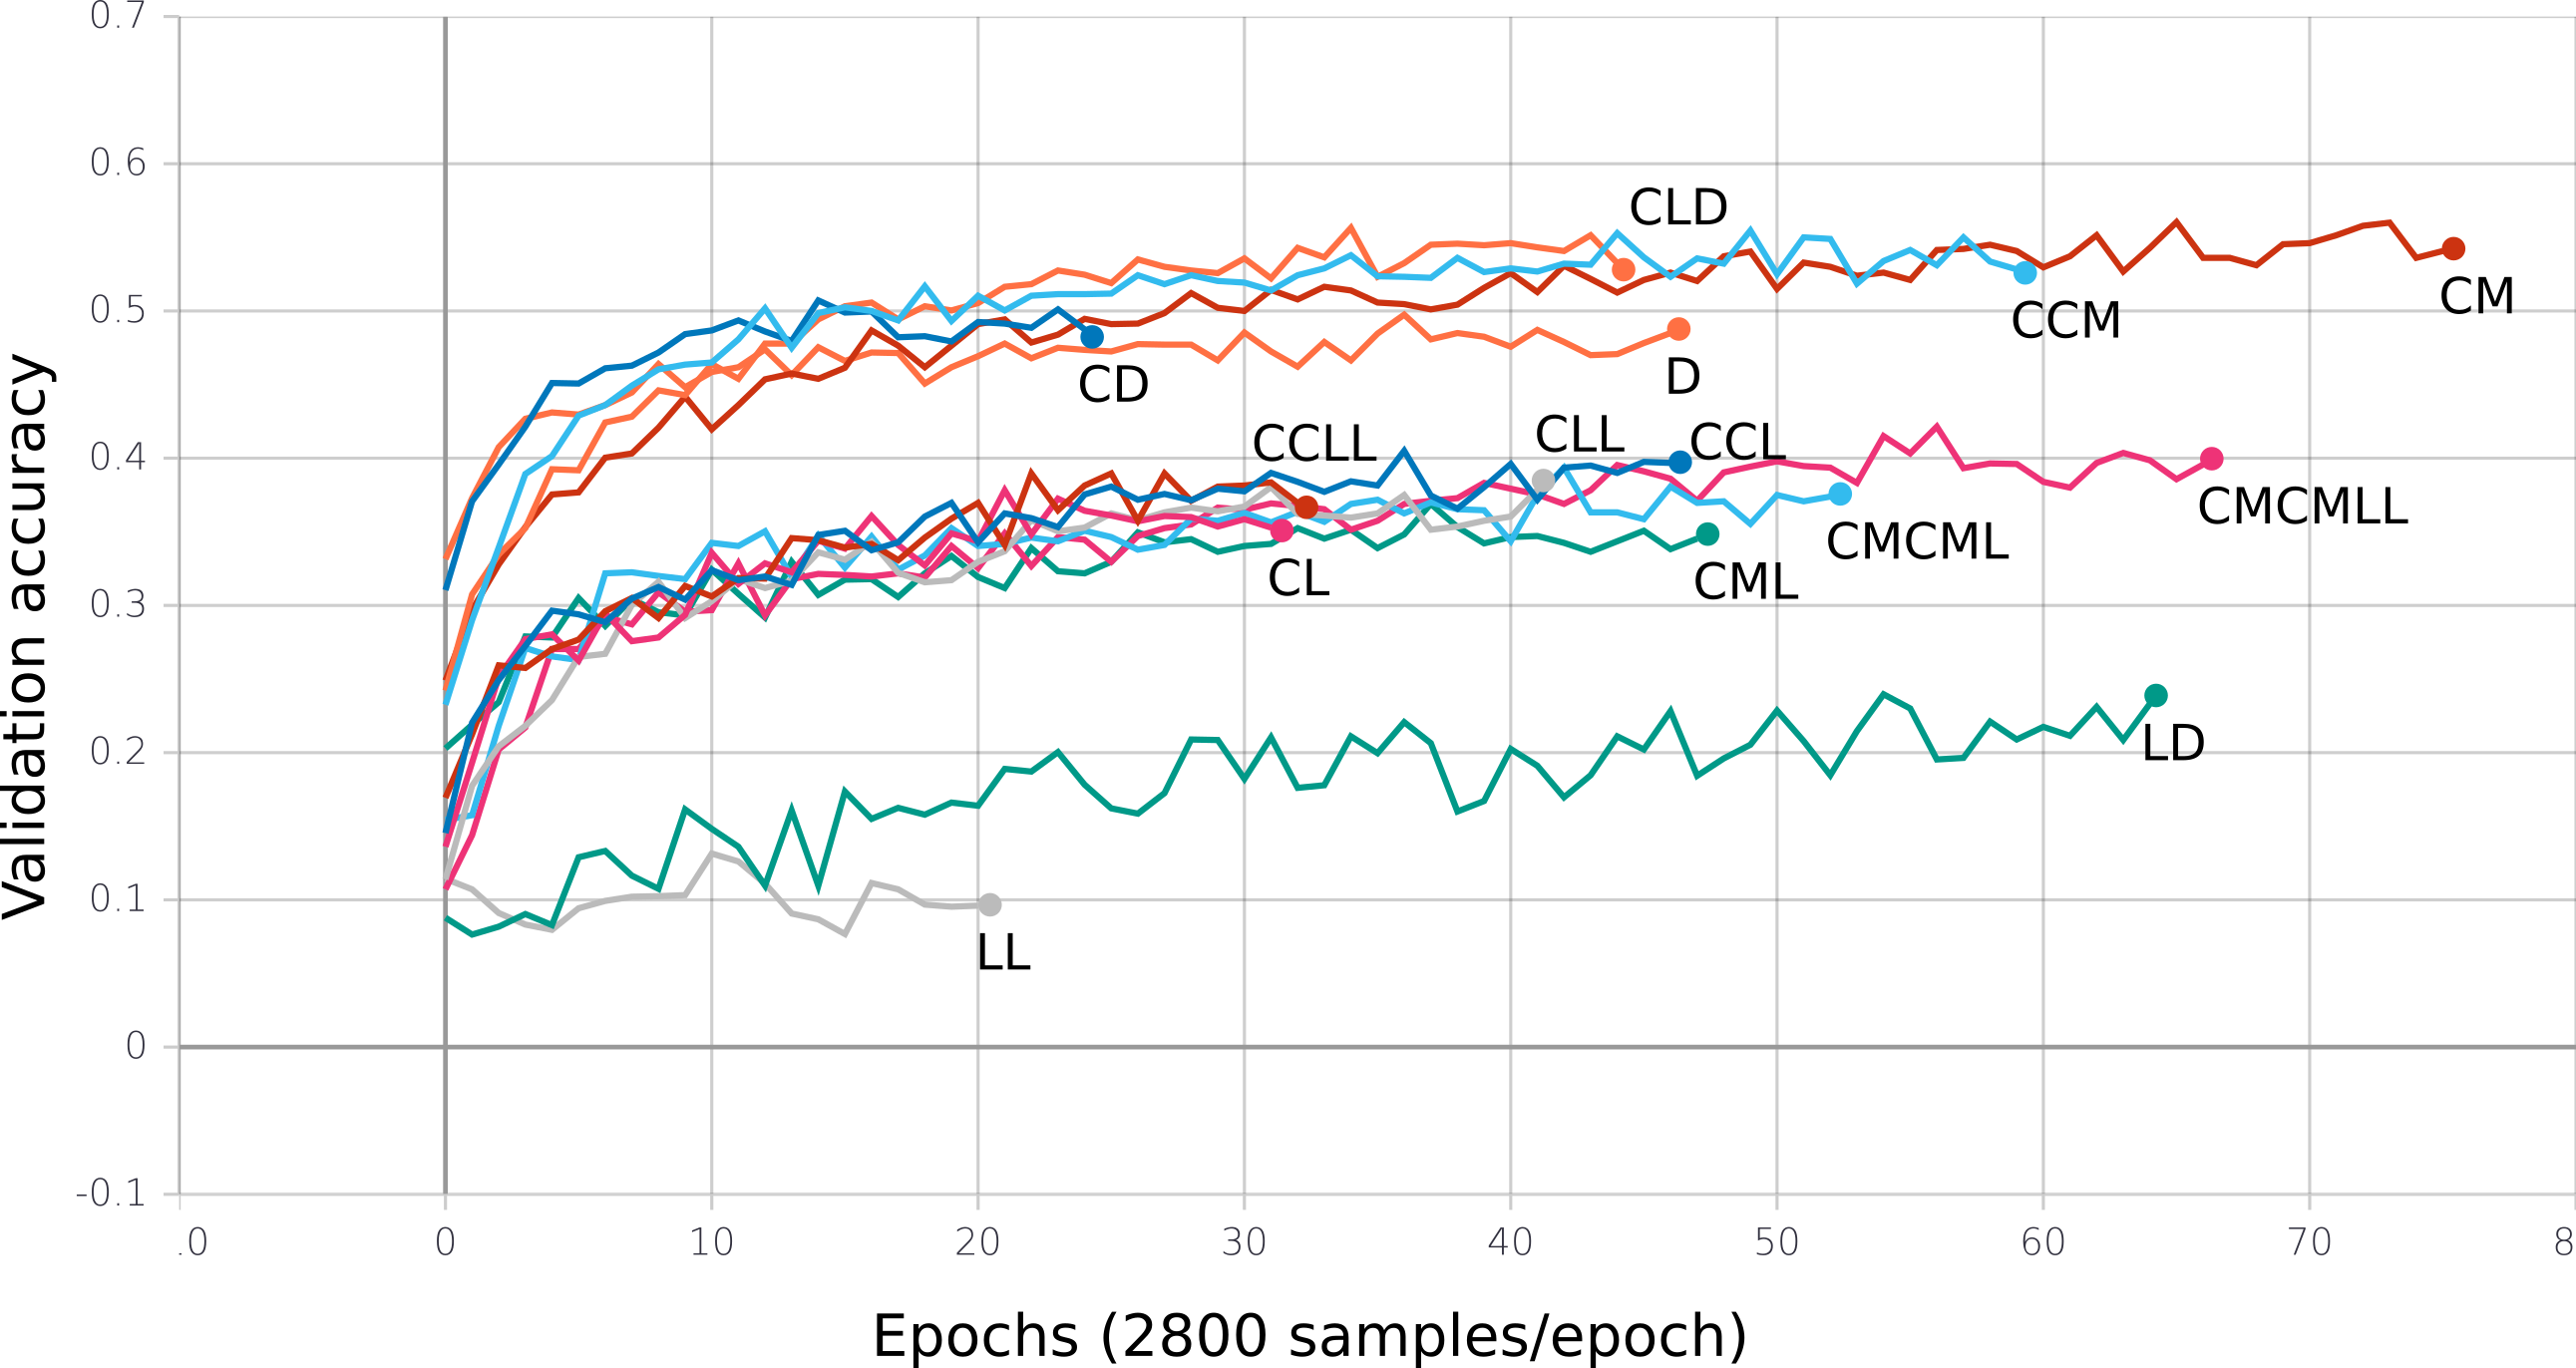
\includegraphics[width=0.9\textwidth]{content/epoch_val_categorical_accuracy.png}
\caption{\label{fig:learning}Learning curves of some models (validation accuracy vs. time)}%
\end{figure*}

%\levelB{Inputs}
%one-hot
The input features of the network for each instance is a 512x256 matrix representing only one block of 512 bytes of a random file of the dataset. Each of the 512 bytes is one-hot encoded, meaning that its value is converted into a vector with 256 elements, with only one of them set to 1, corresponding to the value of the byte, while the others are set to zero. A batch size of 100 was used, with 28 steps per epoch.

%8bits
% The input features of the network for each instance is a 512x8 matrix representing only one block of 512 bytes of a random file of the dataset. Each of the 512 bytes uses a custom encoding where each of the 8 bits of a byte is represented as -1 or 1, depending whether the bit is 0 or 1. During initial tests, this encoding was compared to three other encodings: one-hot encoding, 8 bits represented as 0 or 1\todo{include citation}, and 8 bits represented as [0,1] and [1,0] \cite{hiester_file_2018}. More research should be done in the future to determine the best of the four, but initial results suggest they have similar impact on the model accuracy. The one-hot encoding has the disadvantage of increasing the input matrix size by a factor of 32.

%\levelB{Outputs}
The output of the network for a given instance is a vector with a size equal to the number of classes, subjected to a softmax function, which applies the exponential function on the vector and then normalizes it. Each value will represent the predicted probability that the instance belongs to a specific class.

%exp18
The two models that used LSTM layers without convolutional layers presented slower learning in comparison with the others, as can be seen in figure \ref{fig:learning}. The validation accuracy values can be consulted in figure \ref{fig:models}.


\noindent
\begin{figure*}[htb!]
\centering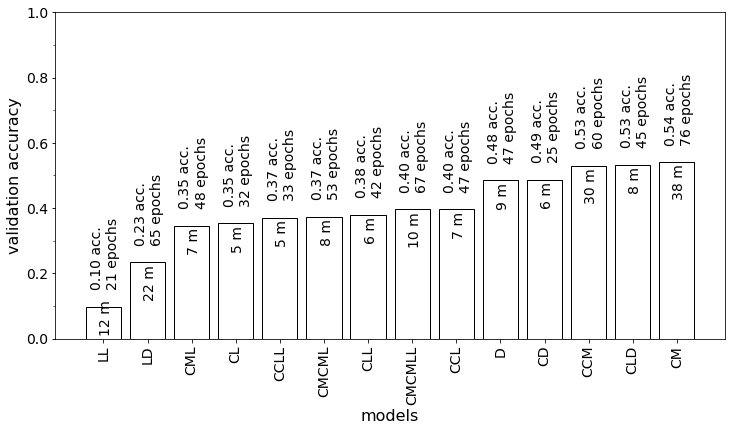
\includegraphics[width=1.0\textwidth]{content/models.png}
\caption{\label{fig:models}The bar plot shows the validation accuracy of the considered models. Their training time, in minutes, and the total epochs processed is also indicated. The training was interrupted when no further improvement was observed for 10 consecutive epochs.}%
\end{figure*}


The validation accuracy values of the remaining models were in the 0.35-0.54 range.

% The selected model for further research, identified as ``CM'', achieved an accuracy of 0.54. The models, ``CLD'' and ``CCM'' achieved similar values, but model ``CM'' performed better in the experiment described in section \ref{sec:exprandom}.

To check if the two slower models could give better results if executed for a longer period, they were trained for 10 hours. The model identified as ``LD'', which uses an LSTM layer followed by a fully connected layer, was able to achieve an accuracy of 0.494, while the other, ``LL'', achieved only 0.153.

%stagnation in learning with such short times, combined with low final accuracy suggests that the dataset present some patterns that are easily recognizable, while the rest of the dataset present a very hard classification task.

% \levelC{Limitations and threats to validity}


\chapter{Conclusion}
The results may be grouped in three groups. The models that used LSTM without a convolutional layer performed poorly. The models with convolutional layers that used LSTM as the final layer had intermediary results. The remaining models were the single layer perceptron (single fully-connected layer model, identified as ``D'') and the models that used convolutional models and used a fully-connected layer or maxpooling as the last layer.

The best accuracy results were from the three models identified as ``CCM'', ``CM'', and ``CLD'', but the latter had faster training time and also showed good resilience to changes: during preliminary tests and later when test conditions where altered to try to improve results, this model and its variations always were among the best models while the others were not.

This study evaluated some alternative models in the file fragment classification task. The expectation was to identify the most promising models for improvement. But an apparent limit was found on how far these models could be improved. 

The anticipation that LSTM models would be a good fit to file fragment classification was contradicted: the results of networks using only LSTM layers without convolutional ones were poor in accuracy and training speed. However, good results were obtained using LSTM as an auxiliary layer to a mainly convolutional neural network (CNN). 

% Using different combinations of layers and parameters, the expectation was that some models would be discarded and some would be selected as promising alternatives. That could be used to guide future researches and also serve as a reference for comparison between studies. 
The Govdocs1 dataset brought an important basis for comparison to be used between carving solutions. But to achieve easily reproducible results, the models must also be publicly available, a condition not all revised studies fulfill. Being available as Jupyter notebooks at https://github.com/atilaromero/carving-experiments, the results described here should require little effort to be reproduced. Thus the source code to generate models with same architecture of those presented here can be used as a basis of comparison in future researches.

A comparison was made between a chosen model, CLD, and recent works on the field. While CLD achieved slight lower accuracy values than the other studies, it can be noticed that the values are very similar. This is a strong indication that the high  variation that those studies show between each other are caused by the difference in the file types they choose. This supports the claim that advances in this area should come from error analysis instead of model tweaking.

\section{Limitations and threats to validity}

In this research, the models were not trained until exhaustion. This was initially done to identify which models would be most promising for future testing, but further attempts to tune layer types, quantity and parameters resulted in accuracy values still close to 0.6, which suggests that selection or tuning of models may not be the best approach to improve results.

However, the 14 models used in this study represent a very small sample of all possible model architectures using the chosen layer types. Moreover, there is no certainty that in different circumstances the best performing models will continue to outperform the others. For those reasons, the search for an alternative model could also be a valid research direction.

The proposed models use a small number of layers. Since deep networks have shown good results in other applications, a study that increase the number of layers of the models presented here may improve results.

\section{Future work}

Most models required short training times and few examples to approach their limit.
This suggests that some patterns were very easy to find but they were insufficient to achieve a higher accuracy.
This raises the question whether there are harder patterns that could be found by a better model not yet tried or if this a more fundamental issue that would not be solved by a trial and error approach of tweaking of parameters and layer modifications.

Based on the work presented here, further studies focused on error analysis are in progress to address this question.
